\documentclass{template/socthesis}

\usepackage{subcaption} 
\usepackage{amsmath} 
\usepackage{enumitem} 
\usepackage{hyperref} % reference
\usepackage{gensymb} % balíček symbolů
\usepackage{booktabs}

\usepackage[toc,page]{appendix}
\usepackage{color} % balíček pro obarvování textů
\usepackage{xcolor}  % zapne možnost používání barev, mj. pro \definecolor
\definecolor{mygreen}{RGB}{0,150,0} % nastavení barev odkazů 
\usepackage{listings} % balíček pro formátování zdrojových kódů 
\usepackage{multirow}
\usepackage{pifont}
\usepackage{pdfpages}
\usepackage[author=,status=draft]{fixme} % vkládání poznámek  
% dva módy (status): draft (poznámky se zobrazují v PDF) / final (poznámky se nezobrazují v PDF)

\newcommand{\cmark}{\textcolor{green}{\ding{51}}}%
\newcommand{\xmark}{\textcolor{red}{\ding{55}}}%

\lstset { %
    language=C++,
    backgroundcolor=\color{black!5}, % set backgroundcolor
    basicstyle=\footnotesize,% basic font setting
}

\addbibresource{text.bib} % soubor s bibliografií
\nocite{*}

\titlecz{Integrace do průmyslu 4.0} % český název práce
\titleen{Integration into industry 4.0} % anglický název práce
\author{Jakub Andrýsek} % jméno a příjmení autora
\field{10} % obor (pouze číslo, zbytek vysází šablona - číslo oboru viz http://www.soc.cz/obory-soc/)
\school{Gymnázium Brno, Vídeňská, příspěvková organizace} % celý název školy
\mentor{Mgr. Jaroslav Páral} % jméno a příjmení školitele
\mentorstatement{Mgr. Jaroslava Párala} % jméno a příjmení ve druhém pádě 

% Změňte, pokud se liší
%\region{Jihomoravský} % kraj
\placefooter{Brno 2021} % místo a rok

% hinty k používání balíčků hyperref, url, hyperlink a hypertarget
% \usepackage{hyperref} % balíček pro hypertextové odkazy
% \url{www.odkaz.cz}
% \href{http://www.odkaz.cz}{Text který bude jako odkaz}
% \hyperlink{label}{proklikávací_text} - odkaz na text 
% \hypertarget{label}{cíl_odkazu} - cíl odkazu 

\begin{document} % konec preambule dokumentu

\maketitle % vysází titulky

\makecopyrightstatement{V~Brně} % místo

% poděkování
\makethanks{Děkuji svému školiteli Mgr. Jaroslavu Páralovi za obětavou pomoc, podnětné připomínky a~hlavně nekonečnou trpělivost, kterou mi během práce poskytoval.}

\pagestyle{empty}

\section*{Anotace}
Cílem mé práce bylo navrhnout ucelený automatický systém monitorující chod pletacích strojů a~přizpůsobit ho co možná nejlépe potřebám výrobní firmy.

Systém jsem navrhoval na míru pro rodinnou firmu na pletení ponožek a v současnosti je schopen v~reálném čase zaznamenávat a~následně odesílat naměřená data ze strojů na server. 
Pro uživatele systém nabízí moderní webové stránky, kde si může naměřená data přehledně zobrazit a~analyzovat.

Systém se skládá ze tří částí. Senzorová část, která je připojená k~pletacímu stroji a~odesílá data.
Dále pak server, který veškerá data zpracovává a~zobrazuje uživateli.
Poslední částí je podpůrný server, který se stará o~aktualizaci a~o~kontrolu správného chodu senzorů.

\subsection*{Klíčová slova}
IoT, ESP32, web, PHP, Nette, databáze, open-source, průmysl 4.0, automatizace, modernizace


\newpage % pokud se anotace vleze na jednu stránku (což by měla), tento rádek zakomentuj

\vspace{20mm}

\section*{Annotation}
% The aim of my work was to design a comprehensive automatic system that monitors the operation of knitting machines and adapt it as best as possible to the needs of the manufacturing company.
The goal of my work was to design a comprehensive automatic system that monitors the operation of knitting machines according to the needs of a manufacturing company.

% I designed a system tailored for a family sock knitting business and is currently able to record and then send measured data from machines to a server in real time. 
I designed a production monitoring system for a family sock knitting business that can record measured data and submit them from machines to a server via the wireless network in real-time.
% For users, the system offers modern websites where they can clearly display and analyze the measured data.
The system offers a modern web-based user interface where the user can clearly display and analyze the measured data in a form of a real-time dashboard, statistic tables and graphs.

% The system consists of three parts. The sensor part, which is connected to the knitting machine and sends the data. 
The system consists of three subsystems - sensors, a main server, and a support server.
% Furthermore, the server, which processes all the data and displays it to the user. The last part is a support server, which takes care of updating and checking the correct operation of the sensors.  
The sensors are connected to the machines and send the data to the main server via WiFi. 
The main server processes all the data and displays it to the user. 
The support server takes care of updating and checking the correct operation of the sensors. 

\subsection*{Keywords}
IoT, ESP32, web, PHP, Nette, database, open-source, industry 4.0, automatization, modernization

\newpage
\pagestyle{plain}

\tableofcontents % vysází obsah

%%% Začátek práce
\setcounter{figure}{0}
\setcounter{table}{0}
\newpage

% zde můžeš s pomocí příkazu \input{cesta k souboru} vložit soubory; doporučuji každou větší kapitolu dát do samostatného souboru pro větší přehlednost

% Úvod práce

% \chapter{Kapitola}
Lorem ipsum dolor sit amet, consectetur adipiscing elit.
Aliquam nunc magna, sollicitudin id leo eu, viverra congue risus.
Aliquam consequat ipsum ut erat placerat consequat nec at diam. 
Aenean est odio, molestie sit amet nunc in, pretium luctus elit. 
Donec imperdiet orci vel porttitor placerat. 
Proin ut hendrerit elit, ultricies accumsan urna. 
Vivamus condimentum lorem viverra lectus finibus, nec volutpat turpis auctor.
Cras quis felis non lorem consectetur interdum eu eu sem. 
Proin sit amet feugiat metus. 
Ut vitae orci a~enim vestibulum porta. 

\fxnote[author=JA]{\textcolor{mygreen}{Muj Komentar}}

\section{Oddíl}
Lorem ipsum dolor sit amet, consectetur adipiscing elit.
Aliquam nunc magna, sollicitudin id leo eu, viverra congue risus.
Aliquam consequat ipsum ut erat placerat consequat nec at diam. 
Aenean est odio, molestie sit amet nunc in, pretium luctus elit. 
Donec imperdiet orci vel porttitor placerat. 
Proin ut hendrerit elit, ultricies accumsan urna. 
Vivamus condimentum lorem viverra lectus finibus, nec volutpat turpis auctor.
Cras quis felis non lorem consectetur interdum eu eu sem. 
Proin sit amet feugiat metus. 
Ut vitae orci a~enim vestibulum porta. 

\subsection{Pododdíl}
Lorem ipsum dolor sit amet, consectetur adipiscing elit.
Aliquam nunc magna, sollicitudin id leo eu, viverra congue risus.
Aliquam consequat ipsum ut erat placerat consequat nec at diam. 
Aenean est odio, molestie sit amet nunc in, pretium luctus elit. 
Donec imperdiet orci vel porttitor placerat. 
Proin ut hendrerit elit, ultricies accumsan urna. 
Vivamus condimentum lorem viverra lectus finibus, nec volutpat turpis auctor.
Cras quis felis non lorem consectetur interdum eu eu sem. 
Proin sit amet feugiat metus. 
Ut vitae orci a~enim vestibulum porta. 

\paragraph{Odstavec}
Lorem ipsum dolor sit amet, consectetur adipiscing elit.
Aliquam nunc magna, sollicitudin id leo eu, viverra congue risus.
Aliquam consequat ipsum ut erat placerat consequat nec at diam. 
Aenean est odio, molestie sit amet nunc in, pretium luctus elit. 
Donec imperdiet orci vel porttitor placerat. 
Proin ut hendrerit elit, ultricies accumsan urna. 
Vivamus condimentum lorem viverra lectus finibus, nec volutpat turpis auctor.
Cras quis felis non lorem consectetur interdum eu eu sem. 
Proin sit amet feugiat metus. 
Ut vitae orci a~enim vestibulum porta. 

\subparagraph{Pododstavec}
Lorem ipsum dolor sit amet, consectetur adipiscing elit.
Aliquam nunc magna, sollicitudin id leo eu, viverra congue risus.
Aliquam consequat ipsum ut erat placerat consequat nec at diam. 
Aenean est odio, molestie sit amet nunc in, pretium luctus elit. 
Donec imperdiet orci vel porttitor placerat. 
Proin ut hendrerit elit, ultricies accumsan urna. 
Vivamus condimentum lorem viverra lectus finibus, nec volutpat turpis auctor.
Cras quis felis non lorem consectetur interdum eu eu sem. 
Proin sit amet feugiat metus. 
Ut vitae orci a~enim vestibulum porta. 

\chapter{Kapitola 2}
Lorem ipsum dolor sit amet, consectetur adipiscing elit.
Aliquam nunc magna, sollicitudin id leo eu, viverra congue risus.
Aliquam consequat ipsum ut erat placerat consequat nec at diam. 
Aenean est odio, molestie sit amet nunc in, pretium luctus elit. 
Donec imperdiet orci vel porttitor placerat. 
Proin ut hendrerit elit, ultricies accumsan urna. 
Vivamus condimentum lorem viverra lectus finibus, nec volutpat turpis auctor.
Cras quis felis non lorem consectetur interdum eu eu sem. 
Proin sit amet feugiat metus. 
Ut vitae orci a~enim vestibulum porta:
\begin{itemize} % odrážkový seznam
    \item lorem
    \item ipsum
    \item lorem ipsum
    \item lipsum
\end{itemize}

\begin{table}[h]
    \centering
    \resizebox{\textwidth}{!}{%
    \begin{tabular}{@{}l|lll@{}}
        & \textbf{Průmyslová řešení} & \textbf{„Kutilská“ řešení} & \textbf{PROTOPlant}                                                                                   \\ \midrule
    \textbf{Dodání}      & Výroba na zakázku          & „Vyrob si sám“             & \begin{tabular}[c]{@{}l@{}}Možnost sestavení přímo doma, \\ nebo dodání \B{hotového} systému\end{tabular} \\
    \textbf{Cena}        & Drahá ($>$~10~000~Kč)      & Levná ($<$~10~000~Kč)      & Kompromis cena -- výkon (již od 2~500~Kč)                                                                               \\
    \textbf{Ovládání}    & Komplexní                  & Jednoduché (většinou)      & Jednoduché                                                                                            \\
    \textbf{Konektivita} & Většinou ethernet          & Často Wi-Fi                & \begin{tabular}[c]{@{}l@{}}Wi-Fi, Bluetooth, \\ možnost přidání podpory Ethernetu\end{tabular}        \\
    \textbf{Řízení}      & PLC                        & Většinou Arduino           & ESP32                                                                                                 \\ \bottomrule
    \textbf{Modularita}  & Ano                        & Ne                         & Ano                                                                                                   \\
    \textbf{Univerzálnost}& Ano                       & Ne                         & Ano                                                                                                   \\ 
    \textbf{Open-source} & Ne                         & Většinou ano               & Ano                                                                                                   \\ \bottomrule    
    \end{tabular}%
    }
    \caption{Tabulka srovnání PROTOPlantu a~jiných řešení.}
    \label{tab:COMPARATION}
\end{table}

\begin{figure}[htbp]
    \centering
    \includegraphics[width=\textwidth]{img/I2C.png}
    \caption{Celý datový přenos po I2C sběrnici. Převzato z~\cite{I2C_specs}}
    \label{fig:I2C-protocol}
 \end{figure}
 
\noindent\B{Lipsum} -- lorem ipsum dolor sit amet, consectetur adipiscing elit.
Aliquam nunc magna, sollicitudin id leo eu, viverra congue risus.
Aliquam consequat ipsum ut erat placerat consequat nec at diam. 
Aenean est odio, molestie sit amet nunc in, pretium luctus elit. 
Donec imperdiet orci vel porttitor placerat. 
Proin ut hendrerit elit, ultricies accumsan urna. 
Vivamus condimentum lorem viverra lectus finibus, nec volutpat turpis auctor.
Cras quis felis non lorem consectetur interdum eu eu sem. 
Proin sit amet feugiat metus. 
Ut vitae orci a~enim vestibulum porta. \newline

\section{Sumarizace}
Nabídka řešení v~tomto oboru je velmi chudá.
Na jedné straně stojí průmyslová řešení, která jsou drahá a~dodávají se primárně do skleníků velkých zemědělských firem.
Na opačném břehu jsou řešení amatérská. 
Ta jsou ovšem buďto naprosto nepoužitelná v~běžně velkém skleníku (primárně je uživatelé vyrábí pro malá pařeniště), nebo neuniverzální.

\newpage

\chapter*{Úvod}
\addcontentsline{toc}{chapter}{Úvod}
Cílem práce je navrhnout ucelený systém monitorující chod pletacích strojů ve firmě a~přizpůsobit ho co možná nejlépe potřebám firmy.

S~nápadem vytvořit takovýto systém přišel můj děda, zakladatel firmy na výrobu ponožek.
Jeho snem vždy bylo mít takový systém, který by částečně zastal monotónní lidskou práci a~nahradil ji efektivní automatizací.

Můj systém jsem tedy navrhoval na míru pro rodinnou firmu na pletení ponožek, ve které je okolo 25 pletacích strojů. 
Tento systém je schopen v~reálném čase zaznamenávat a~následně odesílat naměřená data ze strojů na server. 
Pro uživatele pak systém nabízí moderní webové stránky, kde si může naměřená data přehledně zobrazit a~analyzovat.

Podle pletacích strojů na kterých tento systém běží jsem projekt pojmenoval Pletačka IoT. 
Systém se skládá ze tří částí. Senzorová část, která je připojená k~pletacímu stroji a~odesílá data.
Dále pak server, který veškerá data zpracovává a~zobrazuje je uživateli.
Poslední částí je podpůrný server, který se stará o~aktualizaci a~o~kontrolu správného chodu senzorů.\newline


Při~vytváření tohoto projektu jsem si dal za cíl
\begin{itemize}
    \item projekt s~otevřeným zdrojovým kódem
    \item cenová dostupnost
    \item jednoduché přidání senzorů
    \item přehledné uživatelské rozhraní
\end{itemize}

Pro systém jsem si stanovil tyto požadavky
\begin{itemize}
    \item Počítání upletených ponožek
    \item Zjišťování poruchovosti strojů
    \item Porovnání jednotlivých pracovních směn
    \item Monitorování průběhu výroby
\end{itemize}

\newpage



\chapter{Integrace do průmyslu 4.0}
Pojem Průmysl 4.0 se do České republiky dostal okolo roku 2013 a~od té doby se stále více rozšiřuje v~průmyslových firmách.
Jedna z~klíčových částí je IoT (Internet of Things), neboli internet věcí, který nám zajišťuje vzdálenou kontrolu a~řízení strojů pomocí elektroniky, senzorů a~různých softwarů.
Další vlastností těchto systémů je zaznamenávání a~následné ukládání dat do datových úložišť.
Moderní IoT řídící systémy se snaží proniknou co nejvíce do hloubky a~zpřesnit tak naměřená data, důležitá pro optimalizaci produkce.   

%SECTION
\section{Popis}
Při~návrhu mého systému jsem se snažil řídit těmito zásadami a~navrhnout tak co nejmodernější a~provozně efektivní systém.
Základem bylo zhodnocení stávající situace a~navržení možného řešení.

Jednotlivé problémy neautomatizované výroby:
\begin{itemize}
    \item dlouhá doba stání nečinných strojů při poruše i nedostatku materiálu
    \item neznalost doby nečinnosti stroje
    \item ruční počítání vyprodukovaného zboží
    \item absence historického přehledu produkce
\end{itemize}

%SECTION
\section{Řešení}
Mým řešením je tedy návrh moderního systému, který by celý tento výrobní provoz monitoroval a~zobrazoval jak operátorovi u stroje, tak zaměstnavateli.
Systém umožňuje on line zhodnocení jednotlivých směn a~jejich vzájemné porovnání.
Systém neustále vyvíjím a~rozšiřuji podle potřeb firmy.

Současné funkce systému Pletačka IoT
\begin{itemize}
    \item monitoring chodu každého pletacího stroje
    \item on line hlášení závady na stroji
    \item monitoring provozu firmy
    \item porovnání pracovních směn
    \item počítání upletených ponožek
\end{itemize}



%SECTION
\section{Nasazení}
Tento systém je aktuálně nasazen ve firmě ROTEX Vysočina \cite{ROTEX}, která se věnuje výrobě ponožek. 
Firma pracuje ve dvousměnném provozu a~týdně vyprodukuje v~průměru 12000 párů ponožek. 

% Díky mému systému by se ve firmě dala optimalizovat produkce a~výkon strojů a~tím zefektivnit budoucí výrobu. 
Díky mému systému Pletačka IoT se ve firmě optimalizovala produkce a výkon strojů a tím zefektivnila výroba. 
Toto se podařilo především díky minimalizování času nečinnosti pletacích strojů z důvodu on line hlášení poruch a úsporou času operátora výroby při dřívějším ručním počítáním upletených ponožek. 
Jako bonus navíc systém vyhodnocuje produktivitu každého zaměstnance a jednotlivé směny.


%SECTION
\section{Pletací stroje}


\begin{figure}[htbp]
    \centering
    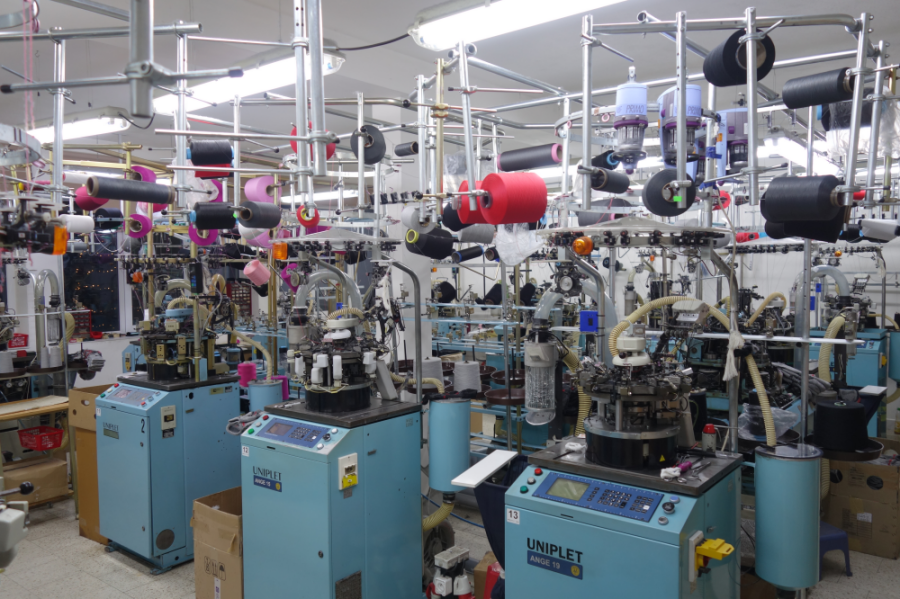
\includegraphics[width=\textwidth]{img/pletarna.png}
    \caption{Pletárna ponožek}
    \label{fig:Pletarna}
\end{figure}

% \begin{figure}[htbp]
%     \centering
%     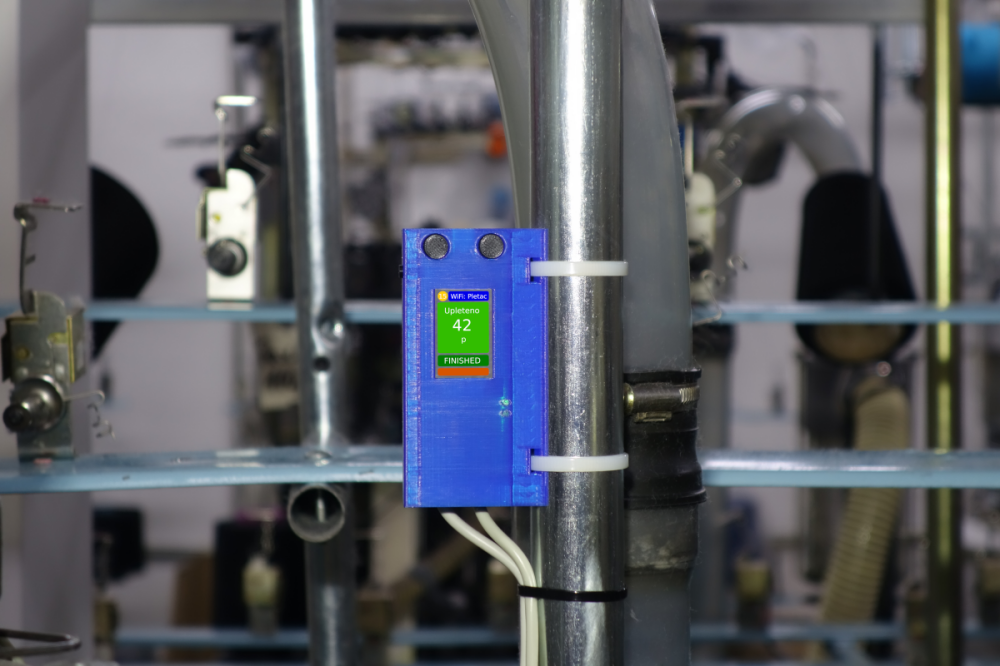
\includegraphics[width=\textwidth]{img/V2-uchyceni.png}
%     \caption{Senzor na stroji}
%     \label{fig:SenzorNaStroji}
% \end{figure}


\newpage


\chapter{Porovnání automatických systémů}
Můj systém Pletačka IoT je velice specifický a~nedá se srovnávat jako celek. 
Potenciální konkurenci tohoto systému jsem tedy rozdělil na dva celky.

\begin{itemize} % odrážkový seznam
    \item Hardwarová část
    \item Softwarová část
\end{itemize}



%SECTION
\section{Hardware}

\subsection{PLC}
PLC neboli programovatelný logický automat je průmyslový počítač k~řízení automatizovaných procesů.
Automaty zpracovávají data v~reálném čase a~s~co nejkratší odezvou.
PLC jsou modulární a~dají se skládat různě dohromady, podle potřeby uživatele.


% \fxnote[author=JPA]{Industruino bych nahradil bych Controllinem: https://www.controllino.com/product/controllino-maxi/}

\subsection{Controllino}
Firma Controllino\cite{CONTROLLINO} se zabývá vývojem zařízení pro průmyslovou automatizaci založenou na platformě Arduino.
Zařízení nabízí několik vstupních a~výstupních pinů, pomocí kterých si uživatel může připojit své senzory a~následně automatizovat některé procesy. 


% \subsection{Industruino}
% Firma Industruino\cite{INDUSTRINO} se zabývá vývojem zařízení pro průmyslovou automatizaci založenou na platformě Arduino.
% Zařízení splňují průmyslové standardy a~jsou navržená pro montáž na  DIN lištu. Firma nabízí také moduly s~WiFi nebo se SIM konektivitou.


\subsection{Hardwario}
Hardwario \cite{HARDWARIO} je česká firma, která nabízí průmyslové IoT stavebnice.
Cílem této firmy je nabídnout průmyslové IoT řešení, které si sami sestavíte podle svých představ.
Firma se zaměřuje na nízkoenergetické moduly s~vydrží několika let.
% Nevýhodou tohoto produktu je jeho vysoká pořizovací cena. 



\subsection{Arduino}
Arduino \cite{ARDUINO} je otevřený (open source) projekt, který se díky své nízké ceně a~jednoduchosti na používání rozšířil po celém světě.
Arduino má v~nabídce přes deset různých modelů. Desky jsou univerzální a~jsou často využívány na kutilské projekty.
K~Arduinu také existuje velké množství shieldů, které základním modulům dodávají další funkcionalitu. 
% Jde například o~WiFi moduduly, motorové moduly, nebo různé teplotní senzory.
Desky Arduino se programují v~jazyce Wiring, vytvořeném přímo pro programování mikrokontrolérů, nebo v~jazyce C++. 




\subsection{Srovnání}

První tří zmíněné platformy jsou hojně využívány v~průmyslu a~řídí většinu automatizovaných procesů. 
Jejich nasazení je složité a~celé systémy jsou velmi drahé.\newline

\newpage

\begin{table}[]
	\centering
	\begin{tabular}{|l|l|l|l|l|l|l|}
		\hline
		\B{Hardware}		& 1 	 & 2 	  & 3 	   & 4 		& 5 	 & 6 	  \\ \hline
		PLC                 & \cmark & \cmark & \xmark & \xmark & \xmark & \xmark \\ \hline
		Controllino         & \cmark & \cmark & \cmark & \xmark & \xmark & \xmark \\ \hline
		Hardwario           & \cmark & \xmark & \cmark & \xmark & \cmark & \xmark \\ \hline
		Arduino             & \xmark & \xmark & \cmark & \xmark & \xmark & \xmark \\ \hline
		\B{Moje řešení} 	& \cmark & \cmark & \cmark & \cmark & \cmark & \cmark \\ \hline
	\end{tabular}
	\caption{Tabulka srovnání hardwarové konkurence.}
	\label{tab:COMPARATION}
\end{table}
	
Požadavky na hardwarovou část
\begin{enumerate}
    \item Připraveno na montáž na zařízení
    \item Průmyslové napětí 5-25 V
    \item Open source
    \item Barevný displej
    \item Bezdrátová aktualizace senzorů
	\item Moderní konektor USB-C
  \end{enumerate}

\newpage

%SECTION
\section{Software}


\subsection{Node-RED}
Node-RED je jednoduché grafické prostředí k~programování IoT zařízení. 
Hlavní výhodou této aplikace je, že celá běží jako webová stránka. 
Tím umožňuje uživateli rychlou práci bez nutnosti instalovat speciální aplikace.
Node-RED programování stojí na principu propojování jednotlivých uzlů.
% Pro složitější projekty může být složité nastavit propojení bloků.
Ve složitějších projektech mohou být ovšem bloky dosti nepřehledné a~složité na úpravu.


\subsection{Blynk}
Blynk je platforma pro vzdálené ovládání IoT projektů.
Základem platformy je jednoduchá mobilní aplikace pro nastavování a~vyčítání dat.
Aplikace nabízí velké množství widgetů, které se připínají na zobrazovací panel.
Na osobní projekty do pěti zařízení je aplikace zdarma, jinak je nutné platit měsíční poplatky.


\subsection{Home Assistant}
Home Assistant je software pro řízení chytrých domácností. 
Systém dokáže pracovat s~více než 1700 službami.
% Připojená zařízení se konfigurují pomocí textového souboru.
Aplikace také dokáže integrovat mnoho rozšíření, například ESPHome.
To slouží k~ovládání mikrokontrolérů ESP které jsou hojně rozšířené v~kutilské komunitě.
% Aplikace také nabízí přehledné widgety k~rychlému zobrazení nejdůležitějších dat. 


\subsection{Porovnání softwarové části}
Node-RED a~Home Assistant jsou projekty s~otevřeným zdrojovým kódem, utvářené komunitou.
Díky tomu jsou tyto systémy modulární a~rychle se rozvíjejí. % přizpůsobují novým zařízením.
Naopak Blynk je uzavřená platforma zaměřená na firmy a~vývojáře.
Můj systém spojuje užitečné vlastnosti ze všech těchto systémů a~nabízí je jako celek v~podobě systému Pletačka IoT.
% Všechny ty tyto platformy pracují s~velkým množstvím různých programovatelných IoT senzorů.


\chapter{Senzory}

Senzory k~projektu Pletačka IoT jsou postavené na mikročipu ESP32 a~modulu TTGO~T-Display.
Celý tento systém je navržen tak, že na každém pletacím stroji je jeden senzor.
Každý z~těchto senzorů má svoje jedinečné číslo, pod kterým posílá naměřená data na server.
Senzor je napájen z~5 nebo 24 voltů a~má spotřebu 120 mA.
Návrh senzorů i~jejich software mám verzovaný nástrojem Git ve veřejném repozitáři~na GitHubu.\newline
GitHub: \href{https://github.com/Pletacka-IoT/Pletacka-board}{Pletacka-board}\cite{PL_BOARD}

\section{Procesor}
Jako řídící procesor jsem zvolil čip ESP32, protože je velice výkonný a disponuje konektivitou WiFi.
Procesor obsahuje 4MB flash paměti sloužící k ukládání programu.

Po prozkoumání trhu jsem našel modul TTGO~T-Display, který kombinuje barevný displej s čipem ESP32.
Tato kombinace mi vyšla jako nejlepší. 
Spojuje bezproblémovou komunikaci čipu s displejem a zároveň jednoduchou výměnu při nefunkčnosti modulu.


\section{Vstupy}
Napájecí okruh pletacího stroje pracuje s napětím 24 voltů, proto jsem potřeboval, aby i moje elektronika, dokázala takovéto napětí zpracovávat.

Jeden vstup je připojen ke světlu které signalizuje zastavení stroje a druhý k senzory, který zaznamenává dopletenou ponožku.
Tyto vstupní signály jsou připojeny na optočleny, které vodivě oddělí vstupní napájení.
Na výstupu máme poté pouze třívoltový signál, který je zpracovatelný čipem.

Jako uživatelské vstupní periferie jsem využil jednoduchá tlačítka, pomocí kterých si uživatel upravuje nastavení senzoru.


\section{Výstupy}
Jako hlavní zobrazovací článek jem využil barevný TFT displej o velikosti 1,14 palce.
Na displeji se zobrazuje číslo zařízení, počet upletených ponožek a doba stání stroje.
Spodní část je vyhrazena na logovací a chybové hlášky.

Druhým výstupním prvkem jsou barevné diody.
Ty využívám k signalizaci funkčnosti senzoru a k 
Ty slouží pro signalizaci odesílání dat a k jednoduchému zjištění funkčnosti celé elektroniky.

\begin{figure}[htbp]
    \centering
    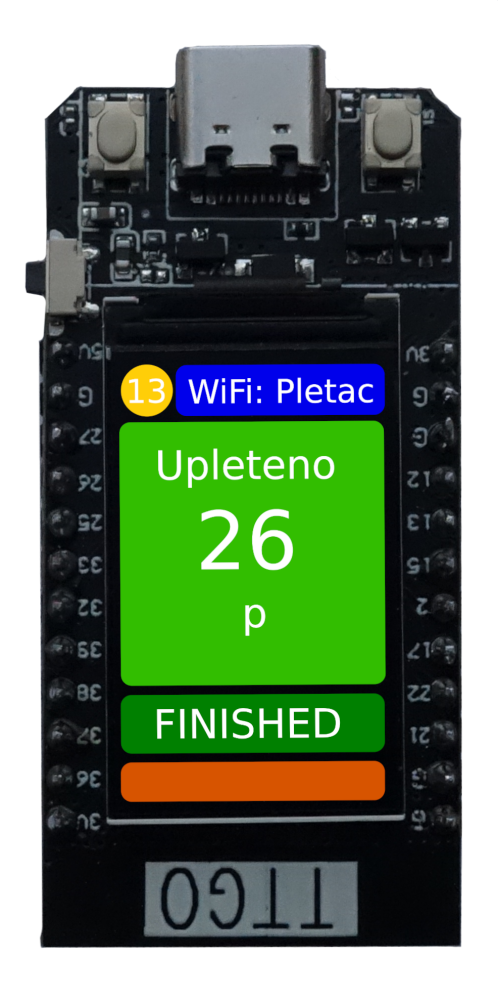
\includegraphics[width=\textwidth/3 ]{img/ESP32.png}
    \caption{TTGO~T-Display}
    \label{fig:TTGO}
\end{figure}


\section{Vlastní PCB}
K vytvoření vlastní desky mě vedlo několik faktorů. První z nich byla velikost celé elektroniky. 
Nevýhodou elektroniky postavené z existujících modulů je právě jejich velikost, moduly se dají jednoduše skládat k sobě, ale zabírají spoustu místa. 
 
% Dalším důvodem je replikovatelnost. Těmito deskami plánuji osadit celou firmu, díky čemuž bylo zapotřebí vyrobit 3O stejných elektronických desek.
Dalším důvodem je replikovatelnost. Těmito deskami plánuji osadit celou firmu, což znamená vyrobit 3O stejných elektronických desek.

Desky jsem si tedy nechával vyrábět v čínské firmě JLCPCB. Jejich výroba je velmi precizní a dokáží desku i osadit vybranými součástkami.



\section{1. verze - univerzální sensorika}

První verzi jsem pojal jako testovací. Bylo tedy třeba navrhnout univerzální desku a~otestovat celý systém.\newline

Při~navrhování senzoru jsem si stanovil tyto body:
\begin{itemize}
    \item ESP32 s~barevným displejem
    \item vstup ze 4 periferií
    \item vstupní napětí od 10 do 25V
    \item teplotní čidlo
    \item tři~barevné diody
    \item čtyři~uživatelská tlačítka
\end{itemize}

% \subsection{Elektronika}
% % Modul TTGO~T-Display jsem zvolil kvůli jeho jednoduché práci s displejem. 
% Modul TTGO~T-Display jsem zvolil z toho důvodu, že má přímo v sobě integrovaný mikročip ESP32.
% Ten je dostatečně výkonný a disponuje konektivitu Bluetooth a WiFi. 

\subsection{Řídící deska}
Návrh desky jsem tvořil v~aplikaci EAGLE od společnosti Autodesk. 
Deska má rozměry 75 na 60 mm a~v~každém rohu má upevňovací otvory.
Kabely se do desky připojují pomocí 5 mm svorkovnice.
Na vstupu napájení je měnič napětí, který pracuje v~rozsahu od 10 do 25 voltů a~na výstupu dává 5V. 

Řídící procesor celé desky je modul ESP32 TTGO T-Display.
Tento čip také zajišťuje WiFi konektivitu s~okolím a~odesílá naměřená data na server.
Pro univerzální detekování vstupů z~periferií se využívají optočleny, které předávají signál do mikroprocesoru.
K~uživatelskému ovládání senzoru jsou zde čtyři~programovatelná tlačítka a~tři~indikační diody.
Aktuální naměřená data se zobrazují na displeji a~informují obsluhu o~zastavení stroje a~počtu upletených párů.
Senzor je také schopen zaznamenávat data ze čtyř vstupů a~teplotu z~teplotního senzoru. Viz obrázek \ref{fig:SenzorV1}.

\subsection{Uchycení}
Krut řídící desky je vytisknutý na 3D tiskárně z~materiálu PETG.
Na přední straně je průhled z~plexiskla na barevný displej a~okolo něj jsou rozmístěná uživatelská tlačítka.
Na boční straně krytu jsou připravené dvě drážky na protažení stahovacích zip pásků pro uchycení na sloupek stroje.
Signálové kabely jsou poté svedeny po konstrukci stroje až k~periferiím.


\subsection{Program}
K~programování využívám aplikaci Visual Studio Code s~rozšířením PlatformIO, která je navržena k~programování mikrokontrolérů. 
Zdrojový kód mám napsaný v~jazyce C++.

Program se skládá z~několika vláken, které se pravidelně spouštějí a~vykonávají.
První a~zároveň nejdůležitější vlákno je senzorové.
Zde se periodicky kontroluje stav periferií a~při~změně se odešle událost na server.
Další vlákno zajišťuje pravidelné vykreslování dat na displej a~zbylá vlákna se starají o~správný chod senzoru.

Software také obsahuje ladící mód, ve kterém si administrátor může zobrazit stav senzoru v~mobilní aplikaci a~jednodušeji tak hledat potenciální chybu.

Celý program jsem napsal objektově orientovaným programováním, díky čemuž je velmi jednoduché měnit například počet vstupních periferií.
Každé nové periferii stačí nastavit správný typ, pin na který je připojena a její název.
Poté už stačí zavolat například vyčítací metodu, která vrátí stav tlačítka.


\begin{figure}[htbp]
    \centering
    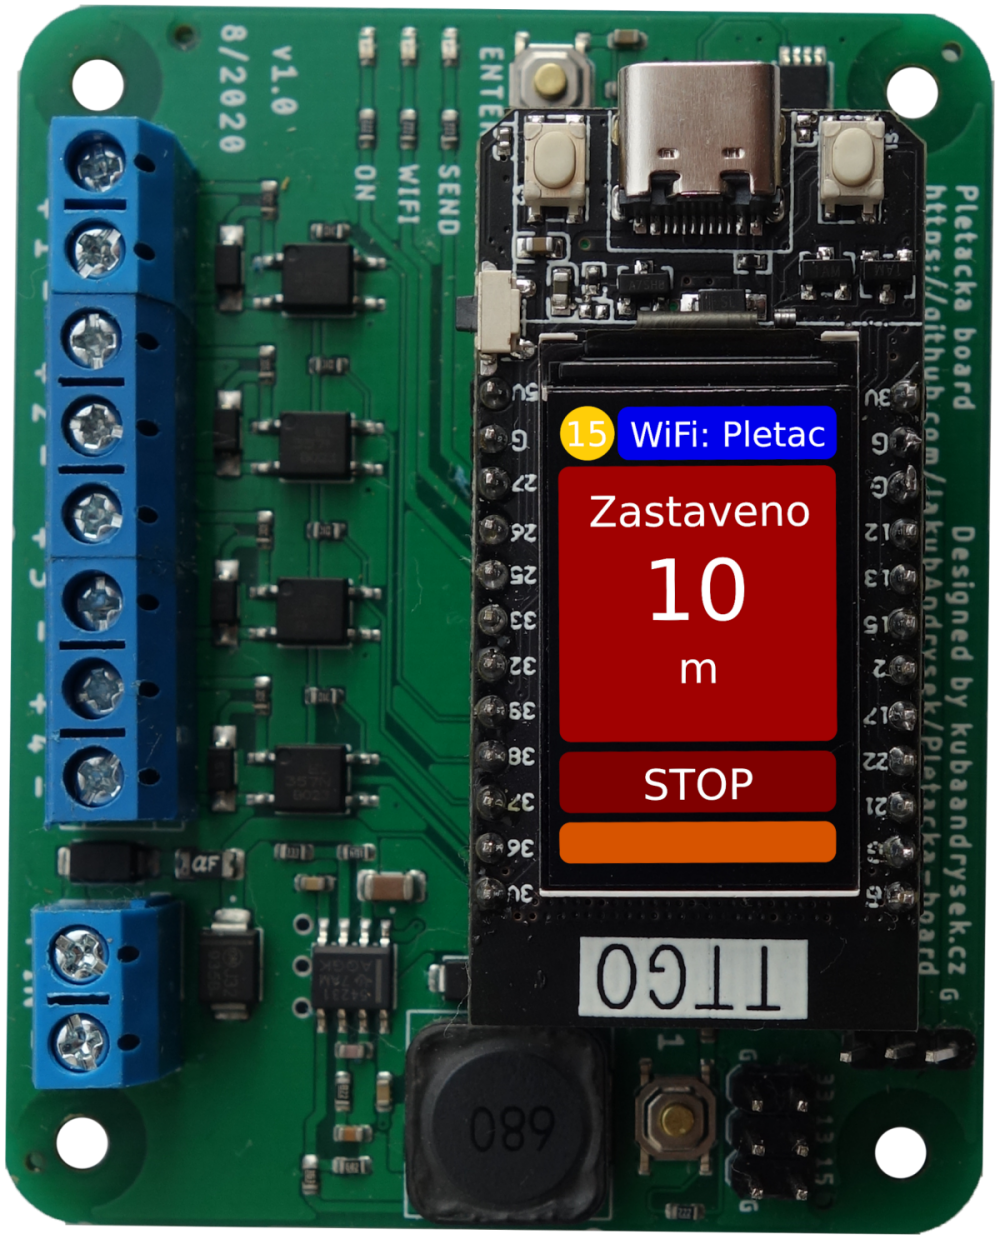
\includegraphics[width=\textwidth/2]{img/V1-deska-esp-screen.png}
    \caption{Senzor - 1. verze}
    \label{fig:SenzorV1}
\end{figure}


\newpage



% 2. verze - speciální senzorika
\section{2. verze - speciální senzorika}

Po měsíci testování jsem zhodnotil využití jednotlivých součástek a~následně jsem vytvořil nový seznam požadavků, přizpůsobený pro lepší chod senzoru.
Zařízení je díky tomu mnohem menší, levnější a~softwarově rychlejší.

\begin{itemize}
    \item vstup pouze ze 2 periferií
    \item vstupní napětí již od 5V
    \item zredukování rozměrů
    \item moderní USB-C konektor
    \item zredukování na dvě tlačítka a~dvě indikační diody
    \item možnost přímého napájení senzoru bez měniče
\end{itemize}

\subsection{Řídící deska}
Návrh druhé desky jsem se rozhodl udělat v~open source aplikaci KiCad.
Z uživatelského hlediska se sní pracuje o něco rychleji díky jednoduchým klávesovým zkratkám. 
Dalším důvodem pro zvolení této aplikace bylo rozšíření KiKit, která razantně zjednodušuje export výrobních podkladů.
Zatímco v dříve používané aplikaci Eagle jsem při každé změně musel projít zdlouhavým procesem exportu, nyní v linuxovém terminálu stačí zavolat `make' a celý proces se vykoná automatizovaně bez nutnosti editace dat.

Rozšíření KiKit jsem také začal používat k automatizovanému generování dokumentace k plošným spojům.
Rozvržení webové stránky si uživatel nastaví v konfiguračním souboru a následně při každé změně se stránka přegeneruje a aktualizuje.

V~novém návrhu jsem se~především zaměřoval na~rozměr desky, ten aktuálně činí 32$\times$76 mm, což je o~46 procent menší plocha než u~první verze.

Deska si~zachovala stejný procesor ESP32 s~displejem, ale přišla~o~dvě~tlačítka a~jednu indikační diodu.
V~senzoru~se také změnilo zapojení měniče napětí.
Nově dokáže pracovat již od~5V, které následně mění na~3,3V.
Na~bočních stranách desky vznikla také nová "křidélka" pro zasunutí~do vylepšeného krytu.



\subsection{Uchycení}
Druhá verze využívá stejného principu uchycení, jako ta~předchozí. 
Mění se~zde však spojení krabičky se~senzorovou deskou. 
V~nové verzi jsem desku navrhl tak, aby se~dala jednoduše zasunout~do kolejnic které jsou předtištěné v~krabičce a~následně zafixovat šroubkem ze~zadní strany.
To~umožňuje jednoduchou montáž~a~rychlé připojení.
Tento návrh už~má~také vyřešené zafixování kabelů ke~konstrukci krabičky pomocí 3D tištěných svěrek.


\subsection{Program}
Program druhé verze vychází z~minulé, ale přináší s~sebou nové funkce a~vylepšuje stávající.
Novou funkcionalitou je například automatická aktualizace programu přes WiFi, kterou nadále zdokonaluji.
Další vylepšení jsem provedl u displeje, který dokáže zobrazit více údajů a~automaticky mezi nimi přepínat.

\begin{figure}[htbp]
    \centering
    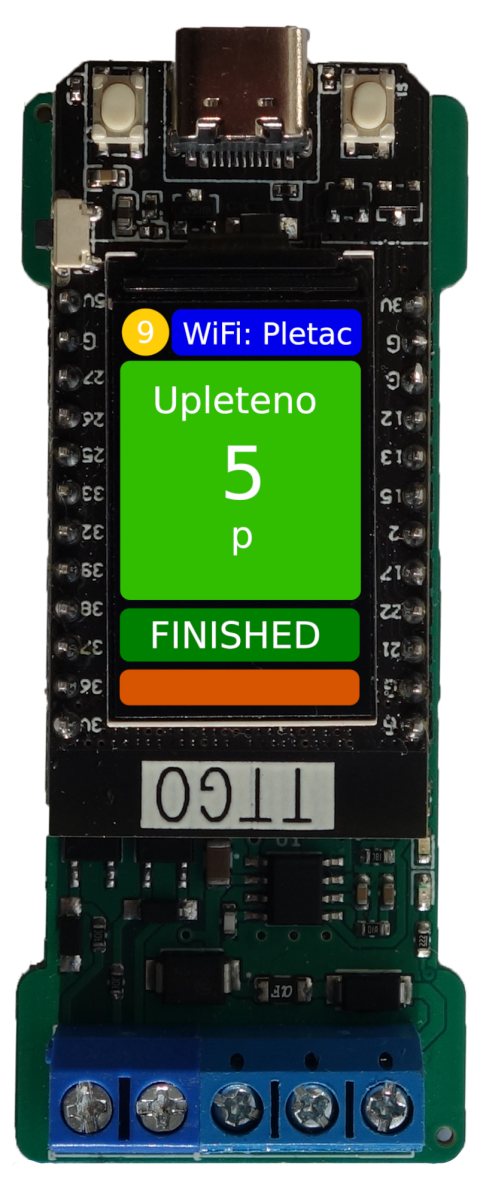
\includegraphics[width=\textwidth/3]{img/V2-deska-esp-screen.png}
    \caption{Senzor - 2. verze}
    \label{fig:SenzorV2}
\end{figure}


\newpage


\chapter{Webový server}
Webový server mám nasazený na mikropočítači~Raspberry Pi 4 Modelu B který, má 8~GB operační paměti.
Toto zařízení jsem zvolil hlavně kvůli nízké spotřebě elektrické energie a~velké komunitě lidí, kteří tento mikropočítač využívají.

Na zařízení běží operační systém Raspberry Pi OS s~grafickým rozhraním.
Webové stránky běží na HTTP serveru Apache2 a~PHP 8.0.
Jako databázový systém využívám MariaDB.
Server běží lokálně uvnitř firmy v zabezpečené síti, díky čemuž je systém rychlý a nezávislý na internetovém připojení.
Celý webový server mám verzovaný také na GitHubu.\newline
GitHub: \href{https://github.com/Pletacka-IoT/Pletacka-website}{Pletacka-website}\cite{PL_WEB}

%SECTION
\section{Frontend}
% Frontend neboli vizuální část webové stránky je pro uživatele ta nejdůležitější.
% Webový design musí zaujmout a~udržet si diváka.
% V~aktuální době plné mobilních telefonů je důležité aby se aplikace správně zobrazovala i~na takto malých zařízeních.
 
Frontend je vizuální část webové stránky zobrazená uživatelem.
Pomocí\newline frontendu se na obrazovku vykresluje veškerý text a~jednotlivé prvky stránky.

\subsection{Bootstrap}
Bootstrap je knihovna sloužící k~jednoduchému a~rychlému vytvoření responzivních webových stránek.
Díky této knihovně jsou stránky správně zobrazovány i~na mobilních zařízeních.
Tento nástroj se vyvíjí od roku 2011 a~je pod otevřenou licencí.
Webový server využívá Bootstrap verze čtyři.


\subsection{JavaScript}
Na frontendu používám JavaScript společně s~technologií AJAX pro aktualizaci částí stránek. AJAX umožňuje překreslovat jen určitou část obsahu stránky bez nutnosti načíst celou stránku znovu.
Tím se zásadně zrychluje načítání a~interaktivita stránek. Dochází i~ke~značné úspoře přenesených dat.
K~tomuto efektivnímu překreslování slouží knihovna Naja\cite{NAJA}, kterou napsal český vývojář Jiří Pudil.
Knihovna také nabízí jednoduchou integraci do PHP frameworku Nette, o~kterém budu psát dále.   



%SECTION
\section{Backend}
Backend je serverová část webových stránek, neběží tedy u~vás~na počítači~jako frontend, ale na webovém serveru.   
Celý backend systému Pletačka IoT jsem napsal v~programovacím jazyce PHP a~ve frameworku Nette\cite{NETTE}, který nabízí ucelenou sadu nástrojů k~tvorbě webu.
Backend se stará o~přijímání dotazů ze senzorů a~následný zápis do databáze, pohání celý webový server a~vytváří databázové výběry.
Nejdříve zde popíšu~použité technologie a~následně rozeberu jednotlivé stránky aplikace.

\subsection{PHP}
Webovou aplikaci programuji v~PHP ve verzi 8.0. Jako programovací studio jsem zvolil studentskou verzi aplikace PHPStorm, která je velmi mocným nástrojem při~tvorbě webu.
Testovací verze aplikace mám spuštěnou na svém počítači,~kde také celý tento systém vyvíjím. 

Pro snadnější ladění chyb používám Xdebug, díky kterému si můžu~krokovat jednotlivé řádky kódu a~rychleji tak nalézt chybu.

Jako systém pro správu balíčků používám nástroj Composer, který se ovládá z~terminálu pomocí jednoduchých příkazů.
Umožňuje rychlou definici závislostí a~aktualizaci všech modulů pomocí jednoho příkazu.


\subsection{Nette}
Nette je webový framework vyvíjený komunitou. Vznikl v~České republice a~jeho zakladatelem je David Grudl. 
Nabízí vlastní šablonovací jazyk, na jednoduché a~efektivní vykreslování webových stránek. 
Nette disponuje obsáhlou a~velmi dobře zpracovanou dokumentací, ale také velkou komunitou lidí, kteří s~tímto frameworkem pracují a~velmi dobře mu rozumí. 


\subsection{REST API}

% REST API je sada příkazů ke komunikaci s~webovou stránkou.
REST API je sada URL identifikátorů sloužících ke komunikaci s~webovou stránkou.
Webová stránka Pletačka IoT obsahuje základní sadu API.
Primárně ji využívají senzory k~odesílání naměřených dat a~ke zpětnému posílání odpovědí do senzoru.
Druhé využití API je k~vytváření databázových výběrů. 
To je voláno nástrojem na automatizaci procesů v~nastavený čas.

%SECTION
\section{Funkcionalita}
Přehled veškerých funkcí mého systému.


\subsection{Podrobné statistiky}
Díky tomuto systému má uživatel kompletní přehled o každém zastavení stroje a upletené ponožce.


\subsection{Aktuální přehledy}
Na úvodní stránce se vždy zobrazují aktuální přehledy o průběhu výroby.


\subsection{Responzivní design}
Stránka využívá moderní CSS styly, díky kterým se stránka správně zobrazuje na jakémkoliv zařízení. 


\subsection{Chytrý výpočetní algoritmus}
Veškerá naměřená data jsou analyzována mým výpočetním algoritmem.
Algoritmus přijímá uložená data z databáze, ze kterých postupným procházením vypočítává pracovní statistiky, které následně ukládá do užších výběrů.


\subsection{Jednoduché grafy}
Většina nasbíraných dat se dá přehledně zobrazit v grafech. 
Díky nim je porovnávání a procházení výběrů velmi jednoduché. 


\subsection{Kontrola běhu stroje}
Prvotním a nejdůležitějším požadavkem systému bylo sledování běhu stroje.
K tomu slouží úvodní stránka aplikace, kde uživatel přehledně vidí ikony všech strojů.
Podle barvy ikony dokáže rozeznat, zda stroj běží, nebo je v poruše a následně si může zobrazit další podrobnosti. 

\subsection{Jednoduchý výběr dat}
Každý senzor nabízí jednoduchý výběr dat.
Uživatel si zvolí požadovaný rozsah dat a aplikace mu tento výběr přehledně zobrazí v tabulce.


\subsection{Porovnávání směn}
Systém jsem navrhoval tak, aby pracoval s dvousměnným provozem a správně přiřazoval data k jednotlivým směnám.


\subsection{Bezpečné zálohy}
Systém se každý den automaticky zálohuje a ukládá data na záložní disk, ze kterého se dají případně rychle obnovit.


\subsection{Jednoduchý generátor zkušebních dat}
Pro otestování systému jsem připravil jednoduchý generátor dat, který dokáže simulovat reálné senzory.



%SECTION
\section{Webové rozhraní Pletačka IoT}
Každá stránka je rozdělena na tři~části. První je záhlaví, které obsahuje logo a~odkazy na nejpoužívanější stránky.
Druhou částí jsou samotné webové stránky které budou popsány v~dalších odstavcích.
Poslední částí je minimalistické zápatí s~copyright znakem.\newline
Stránky Pletačky jsem navrhoval tak, aby splňovaly tyto parametry:

\begin{itemize}
    \item jednoduché rozhraní pro uživatele
    \item přehledné zobrazení dat
    \item zobrazovat pouze užitečná dat
    \item rychlá editace senzorů
    \item využití číselných identifikátorů
\end{itemize}


\subsection{Úvodní stránka}
V~horní části úvodní stránky se vypisují tři~nejpodstatnější údaje.
Jde o~celkový počet upletených párů za aktuální směnu.
Dále pak úspěšnost vypočítávanou z~času zastavení stroje a~z času zapnutí stroje.
Posledním údajem je průměrná doba stání jednoho stroje.   

Pod těmito čísly se zobrazuje tabulka s~barevnými obdélníky, kde každý představuje jeden stroj.
Barva obdélníků udává aktuální stav stroje a~text v~pozadí tuto informaci doplňuje. 

\begin{figure}[htbp]
    \centering
    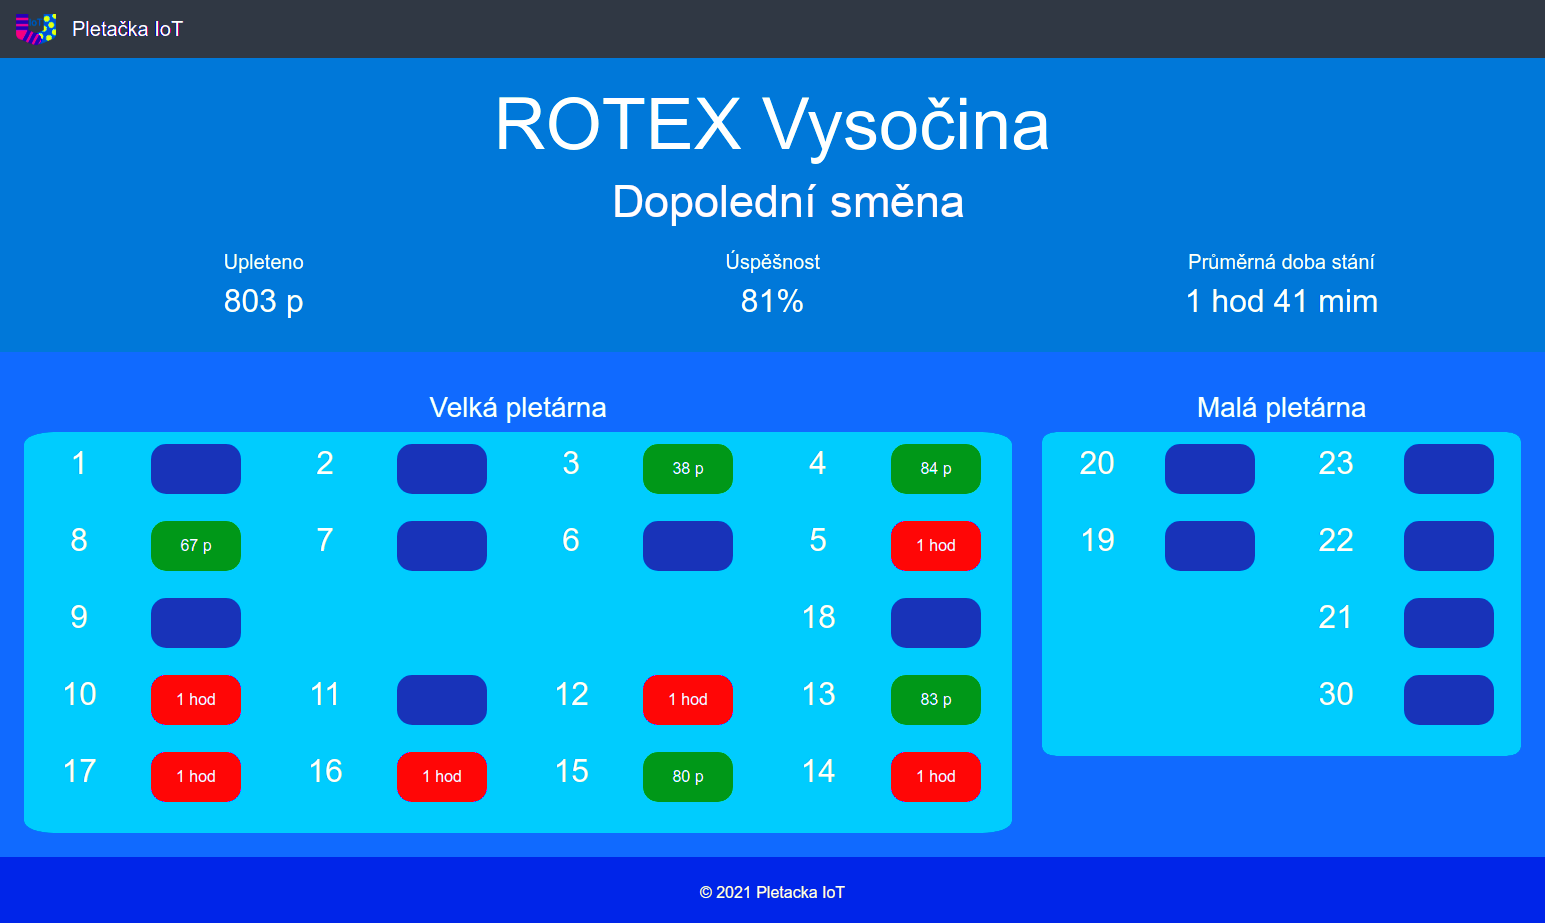
\includegraphics[width=\textwidth]{img/Uvod.png}
    \caption{Úvodní stránka}
    \label{fig:webUvod}
\end{figure}

\subsection{Přehled ze senzoru} 
Po kliknutí na senzor na úvodní stránce se zobrazí data o~právě vybraném stroji.
Veškerá data jsou rozdělena do dvou sloupců podle pracovních směn.
To umožňuje zaměstnavateli jednoduché porovnávání pracovních směn.
V~úvodu každého sloupce je obecný přehled naměřených dat za různá období.
Pod nimi je přehled v~grafech a~porovnání nejdůležitější údajů.

\begin{figure}[htbp]
    \centering
    % 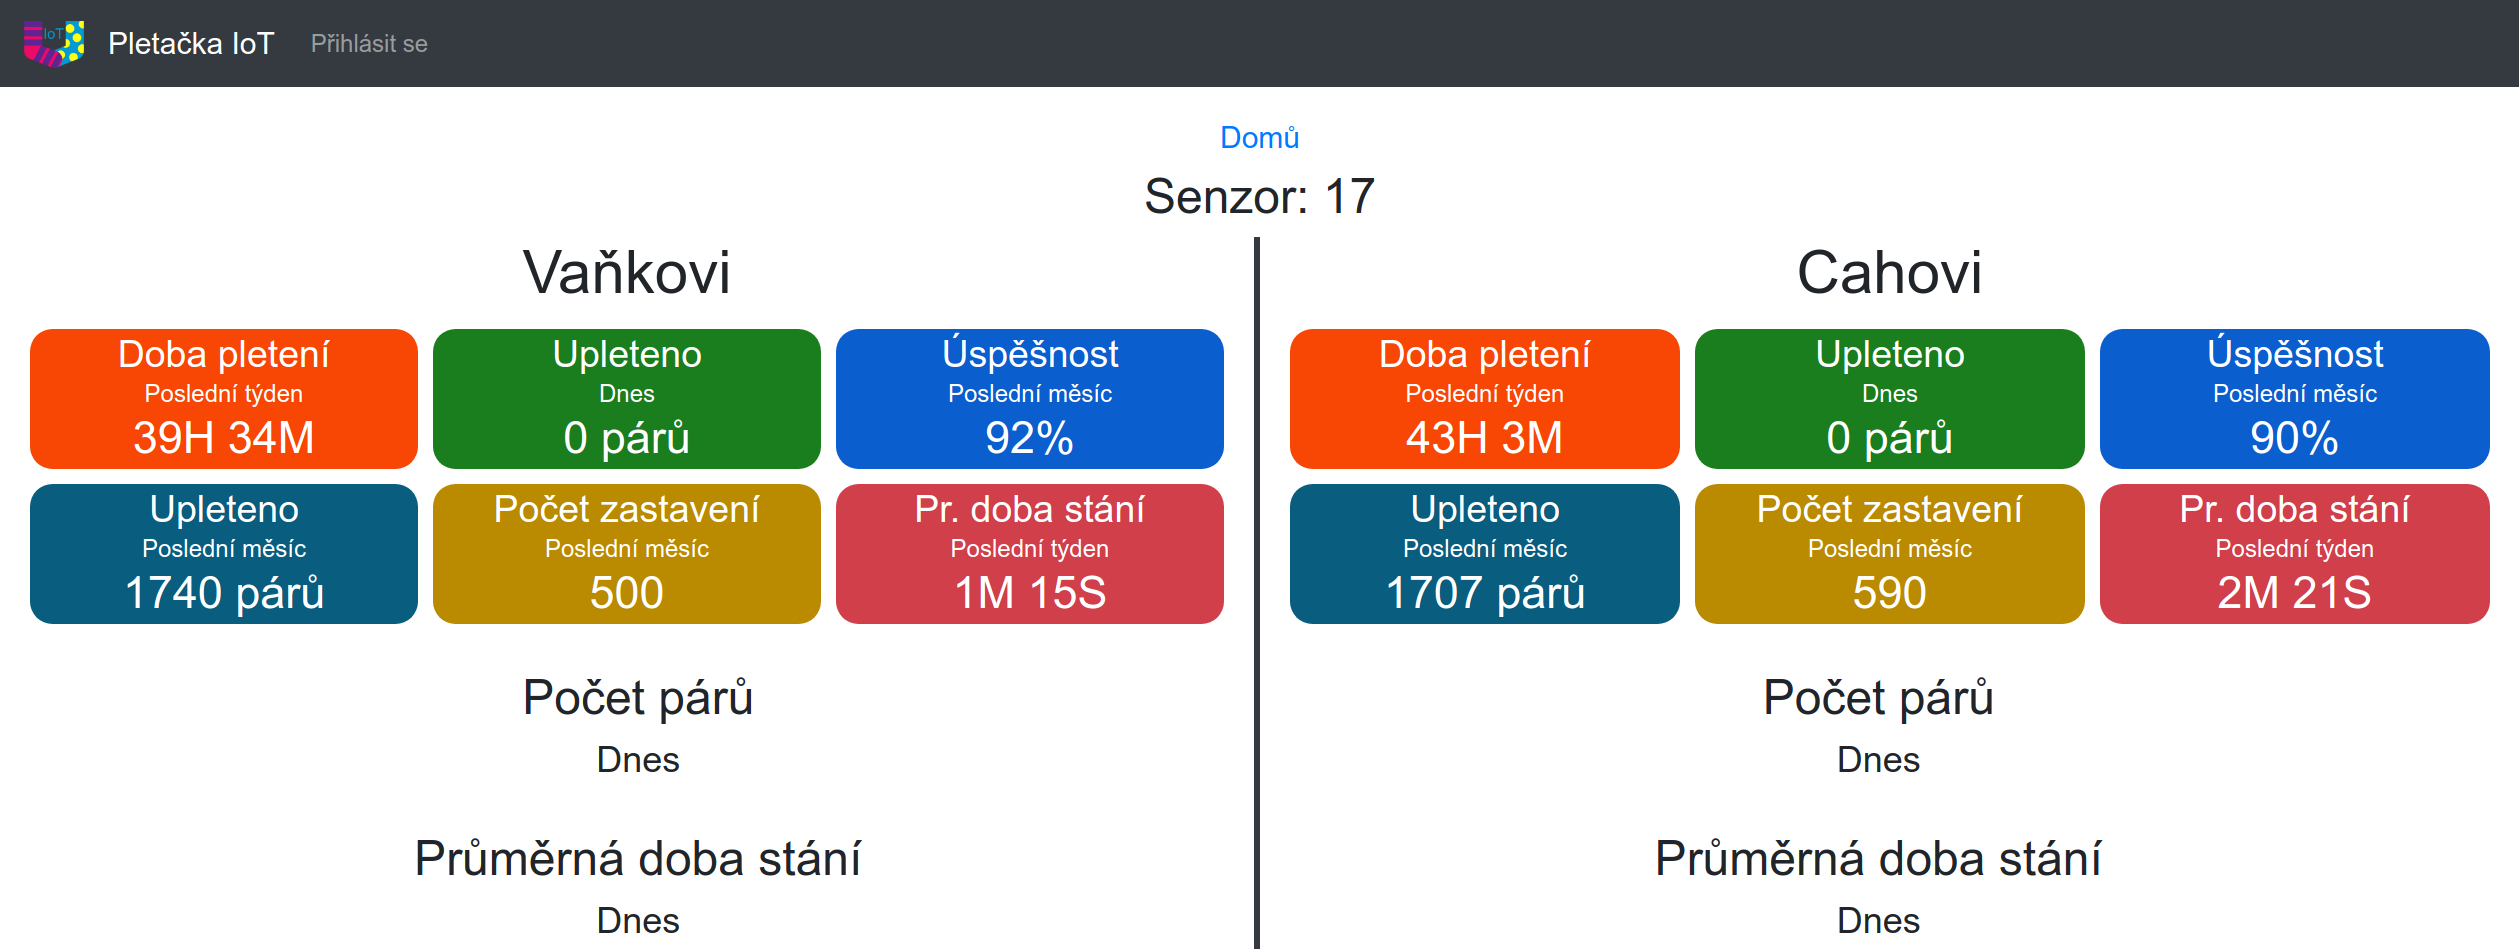
\includegraphics[width=\textwidth]{img/Senzor.png}
    % 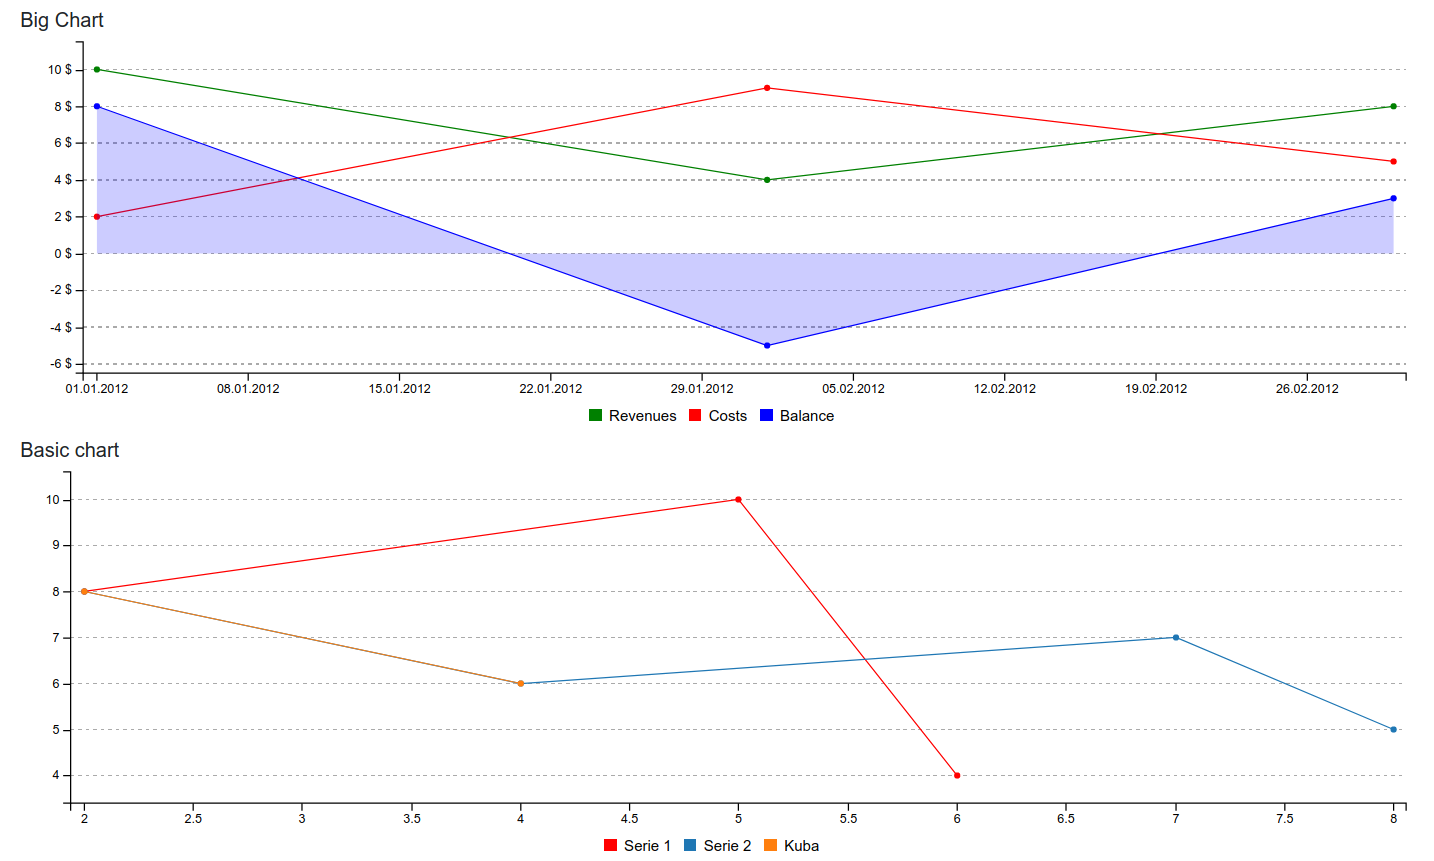
\includegraphics[width=\textwidth]{img/Graf.png}
    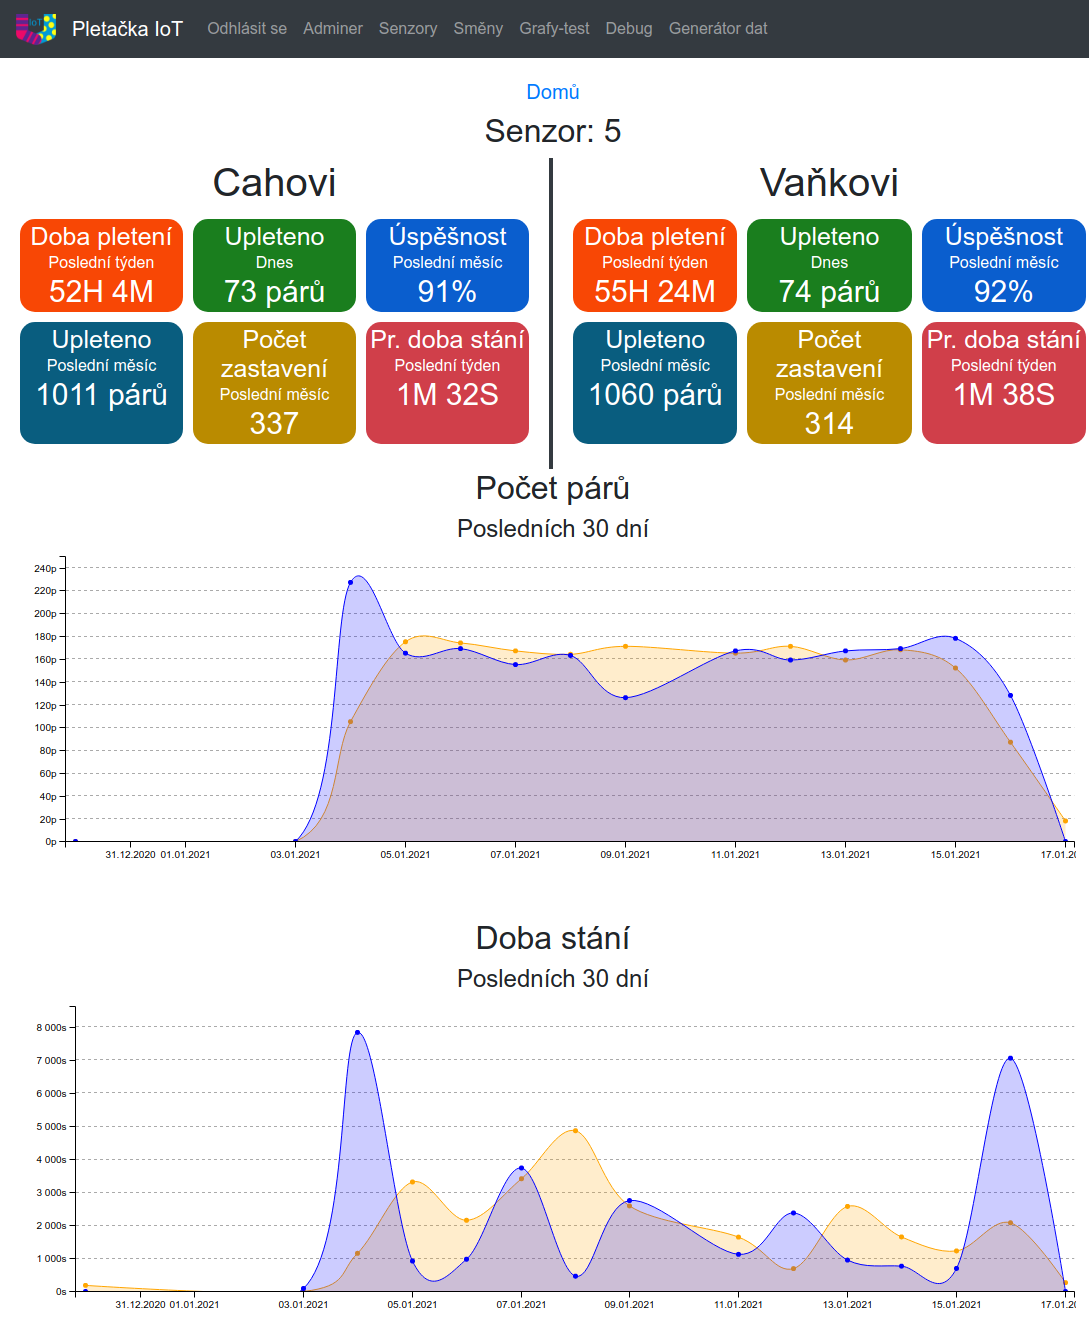
\includegraphics[width=\textwidth]{img/prehled.png}
    \caption{Přehled ze senzoru}
    \label{fig:webSenzory}
\end{figure}


% \fxnote[author=JPA]{\textcolor{mygreen}{Aktualizovat grafy/obrázky}}


\subsection{Správa senzorů}
Pro vstup do této sekce je nutné uživatelské přihlášení do systému.
Stránka pak nabízí přehled senzorů s~jednotlivými možnostmi úpravy (viz obrázek \ref{fig:webSpravaSenzoru}).

% První z~odkazů vede na aktuální přehled ze senzoru.
% Druhý řeší editaci senzoru a~poslední maže vybraný senzor.
% \fxnote[author=JPA]{\textcolor{mygreen}{"První z~odkazů vede na aktuální přehled ze senzoru. Druhý řeší editaci senzoru a~poslední maže vybraný senzor." = není to dostatečně jasné}}

\begin{figure}[htbp]
    \centering
    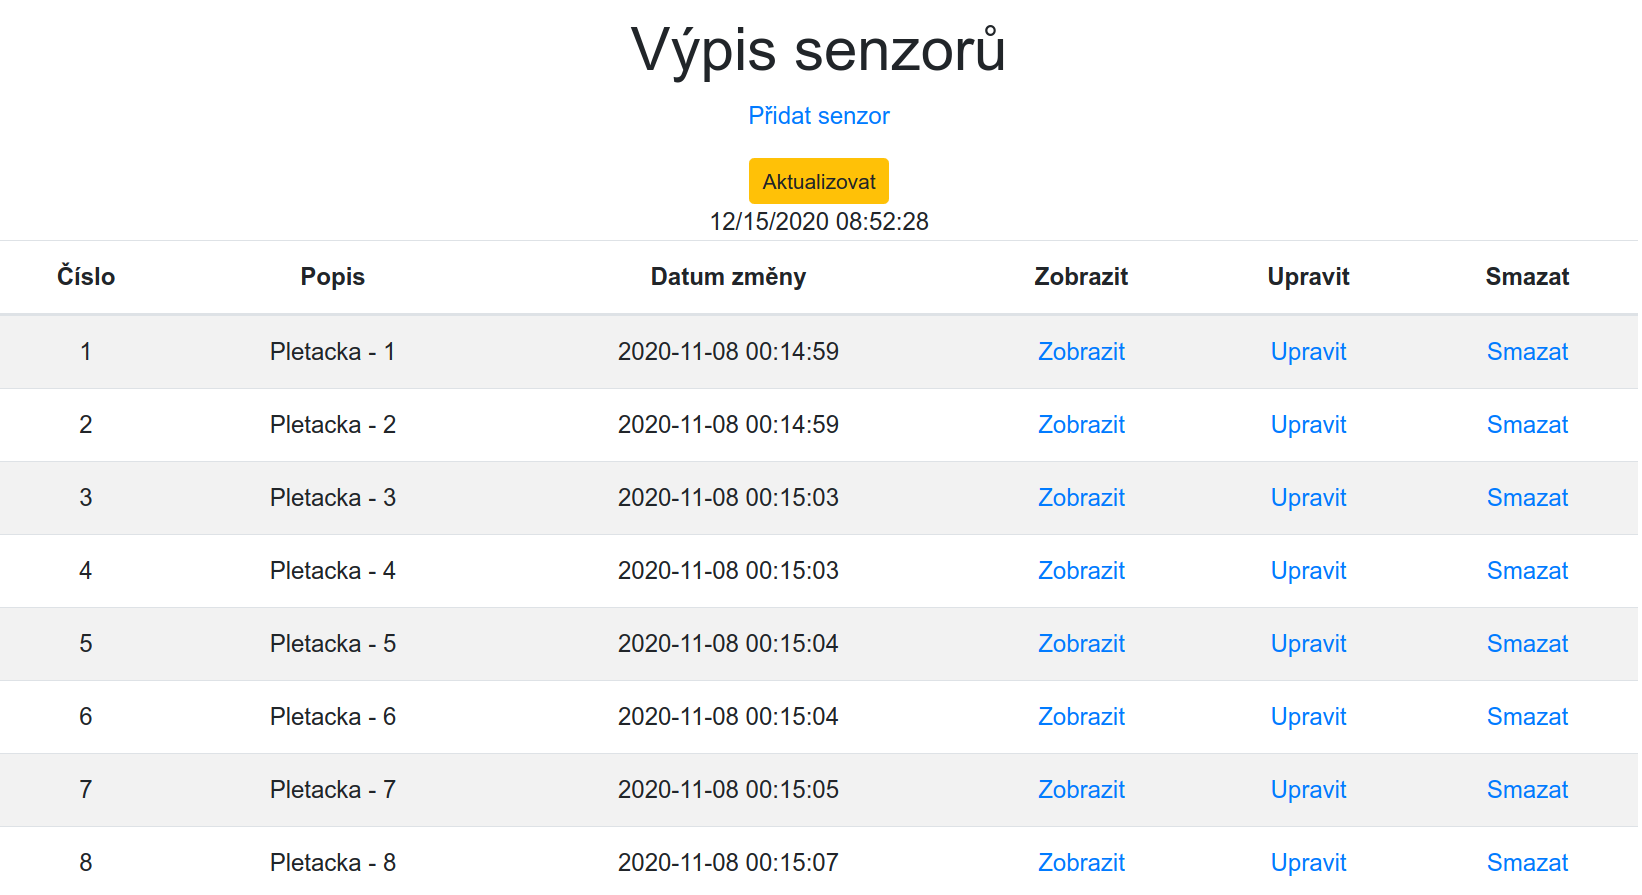
\includegraphics[width=\textwidth]{img/Edit.png}
    \caption{Správa senzorů}
    \label{fig:webSpravaSenzoru}
\end{figure}

\subsection{Nastavení směn}
Jednoduchá stránka na které se nastavuje pořadí směn.
Střídání směn probíhá pravidelně po týdnech, proto je nastavení velmi jednoduché (viz obrázek \ref{fig:webSmeny})

\begin{figure}[htbp]
    \centering
    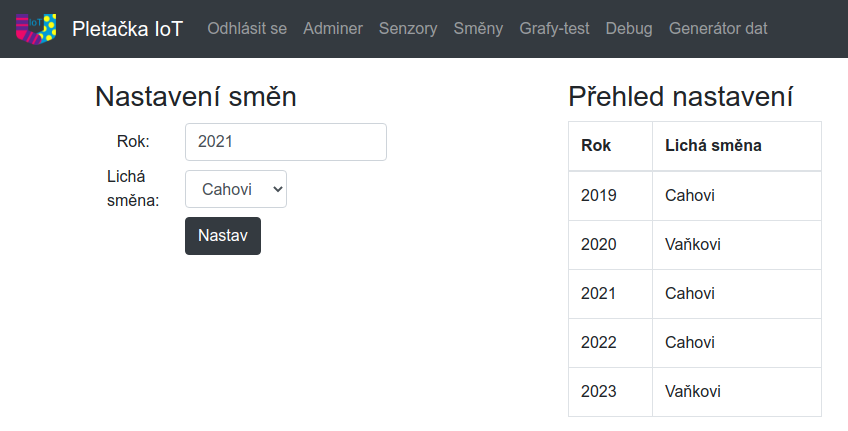
\includegraphics[width=\textwidth]{img/smeny.png}
    \caption{Nastavení směn}
    \label{fig:webSmeny}
\end{figure}

%SECTION
\section{Databáze}
Databáze je rozdělená do dvou skupin tabulek.

První skupina tabulek je nastavovací.
Jedná se o ~tabulku s nastavením senzorů, nastavení směn a~o~tabulku s~uživateli a~jejich oprávněním.

Druhá skupina je senzorová.
Každý senzor zde má pět tabulek na ukládání svých dat.
První senzorová tabulka ukládá čistá nezpracovaná data posílaná přímo ze senzoru.
Zbylé čtyři~tabulky jsou databázové výběry různých časových úseků.
Jde o~výběr hodinový, denní, měsíční a~roční.  
Tyto tabulky se vytvářejí automaticky pomocí výběrového API. 
Struktura tabulek je vyobrazena ve schématu \ref{fig:databaze}.


\begin{figure}[htbp]
    \centering
    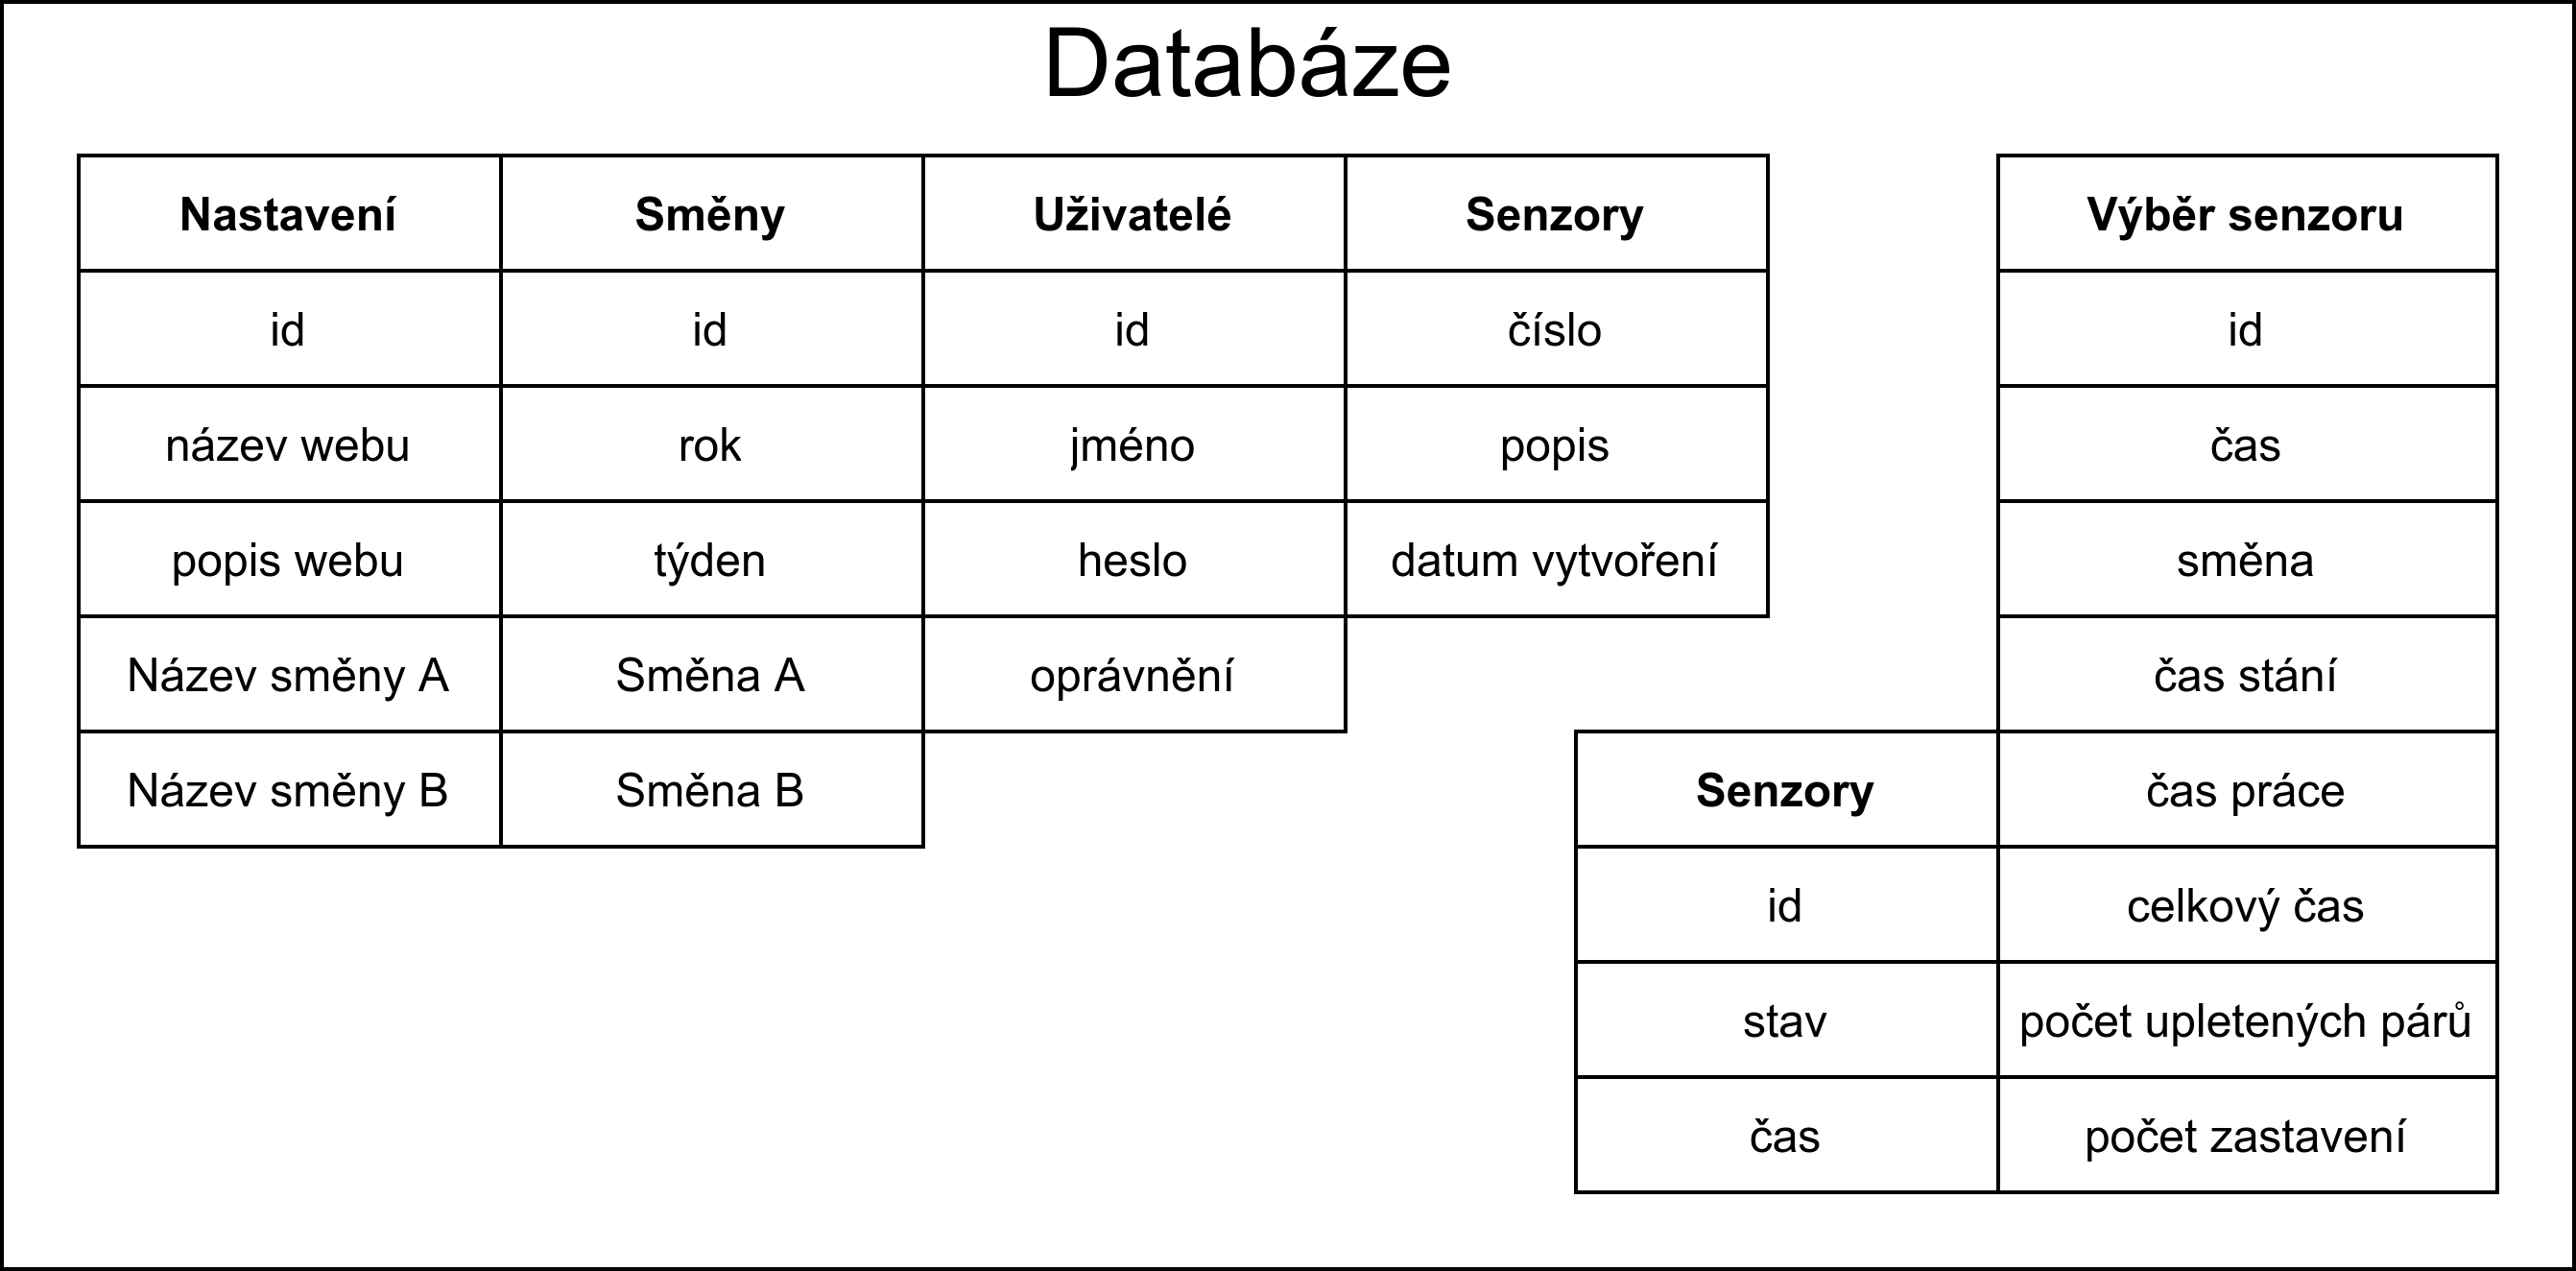
\includegraphics[width=\textwidth]{img/Databaze.png}
    \caption{Struktura databáze}
    \label{fig:databaze}
\end{figure}


\newpage

 
\chapter{Podpůrný server}
Podpůrný server vznikl jako rozšíření pro senzory.
Server je naprogramovaný v Pythonu a běží na Raspberry Pi společně s webovým serverem.\newline
Zdrojový kód na Githubu: \href{https://github.com/Pletacka-IoT/Pletacka-python-server}{Pletacka-python-server}\cite{PL_PY}


%SECTION
\section{Kontrola senzorů}
Hlavním úkolem tohoto serveru je detekce zapnutých senzorů.
Na serveru běží takzvaný Watchdog, jde o hlídacího psa, který každé čtyři vteřiny čaké na zprávu ze senzoru.
Touto zprávou se senzor nahlásí, že je zapnutý, pokud takováto zpráva nedojde deset vteřin, je senzor prohlášen za vypnutý a v databázi se označí jako neaktivní.
Tato jednoduchá metoda umožňuje kontrolovat velké množství senzorů jednoduchým programem.

%SECTION
\section{Automatické aktualizace}
Bezdrátová aktualizace senzorů je nová funkcionalita kterou nadále vyvíjím a rozšiřuji.
Senzory aktuálně podporují rychlou aktualizaci přes WiFi ze vzdáleného počítače.
V počítači stačí vybrat číslo senzoru a nová verze programu se pomocí WiFi připojení nahraje do senzoru.

V nové verzi přibude také hromadná aktualizace senzorů a systém na udržování aktuálních verzí systému ve všech senzorech.




\newpage


\chapter{Princip fungování Pletačka IoT}
V předchozích kapitolách byly popsány jednotlivé část systému Pletačka IoT.
V této kapitole bude celý systém popsán jako celek.


\fxnote[author=JPA]{\textcolor{mygreen}{proč jsou zde "subsection" a ne "section"?}}


\subsection{Sběr dat}
První, a tou nejdůležitější částí, je získávání dat pomocí senzorů.
Jakmile senzor zaznamená jakoukoliv změnu, okamžitě tuto zprávu odesílá na server.
Odesílání probíhá skrze senzorové API, kde se nejdříve senzor ověří a následně se stav zapíše do databáze k příslušnému senzoru.
Po zapsání do databáze se vrátí do senzoru zpráva o provedení zápisu. 


\subsection{Vyhodnocování dat}
Dalším krokem je zpracovávání surových dat z databáze.
K tomuto účelu běží na serveru výběrové API, které je automaticky spouštěné v nastavený čas.
Jde o generování širších výběrů dat, hodinové, denní, měsíční a roční výběry.
Tyto výběry se následně ukládají do databáze k danému senzoru.
Generování těchto dat probíhá převážně v noci, kdy je server nejméně vytížen.


\subsection{Zobrazování dat}
Posledním krokem je zobrazení dat uživateli.
Je to jediná část, se kterou se běžný uživatel dostane do kontaktu.
Proto je nutné, aby zobrazení bylo co nejrychlejší a pro uživatele co nejpříjemnější.
K rychlému zobrazování se využívají předgenerované výběry, ke kterým se rychle dopočítají nově nasbíraná data.


\fxnote[author=JPA]{\textcolor{mygreen}{"se rychle dopočítají nově nasbíraná data" - jaká data se dopočítávají => vice rozepsat}}


\fxnote[author=JA]{\textcolor{mygreen}{schéma sběr - vyhodnocení - zobrazení}}

\begin{figure}[htbp]
    \centering
    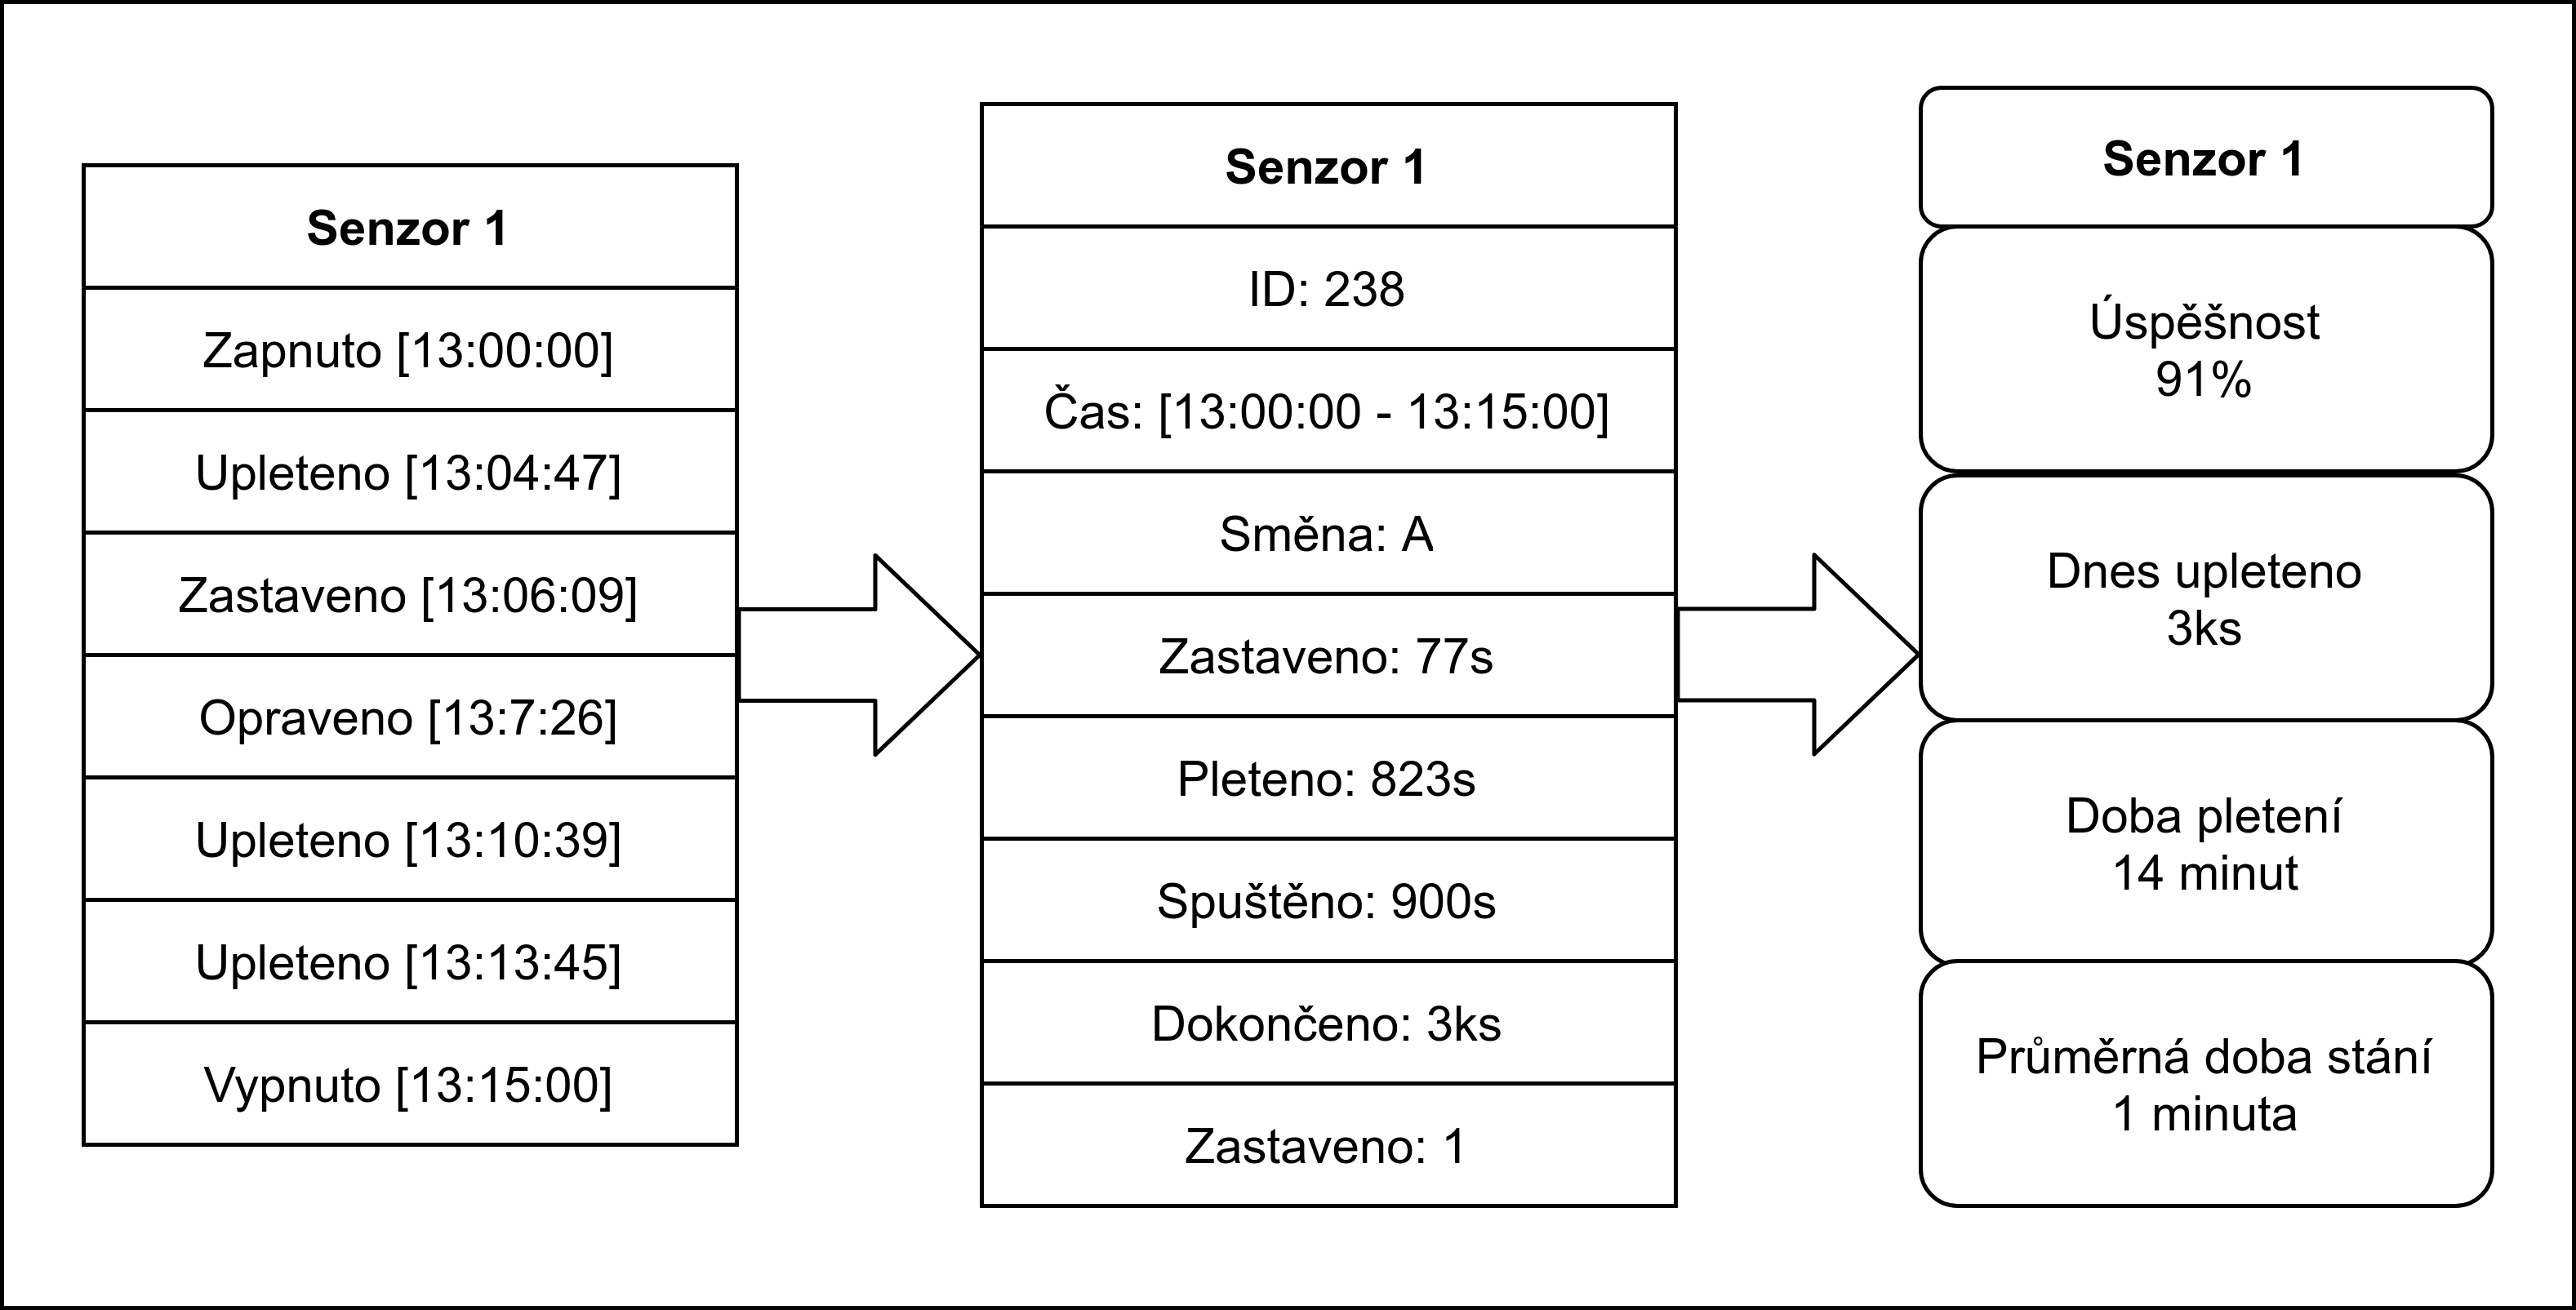
\includegraphics[width=\textwidth]{img/Princip.png}
    \caption{Zpracování dat}
    \label{fig:princip}
\end{figure}

\subsection{Konektivita}
Webové stránky se dají jednoduše zobrazit na počítači či notebooku.
Stránky jsou responzivní a lze je používat i na mobilních zařízeních.
Přístup k webu je pouze z vnitřní sítě firmy, to zajišťuje základní bezpečnost pro systém.


\newpage


\chapter{Vývoj}
Na této práci jsem začal pracovat v únoru 2020, kdy jsem si jako úplný nováček četl dokumentaci k jazyku PHP. 
Původní verzi webového rozhraní jsem začal navrhovat v čistém PHP. Tento způsob byl však velmi zdlouhavý a neefektivní.
Po měsíci práce v čistém PHP jsem přešel na framework Nette, který mi práci zjednodušil a posunul mě velmi rychle dál. 


%SECTION
\section{Systém Pletačka IoT verze 1.0}
Tato verze byla vydána začátkem července, kdy už systém uměl pracovat s virtuálními senzory.


\subsection{Senzory}
Souběžně s programováním webu jsem pracoval na softwaru pro senzory.
V této době byly senzory schopné posílat data na server, ale neměli žádný grafický výstup ani nepodporovaly interakci s uživatelem.

\subsection{Web}
Vznikla základní kostra webu a postupně vznikaly první stránky.
Data ze senzorů se zatím pouze ukládala do databáze a web s nimi zatím neuměl pracovat.
Začínal se vyvíjet systém na zpracovávání údajů ze senzorů.


% \newpage

%SECTION
\section{Systém Pletačka IoT verze 2.0}
Druhá verze přinesla velké rozšíření systému.
% Tato verze byla vydána v půlce prosince a prošla dlouhodobým testováním.
Tato verze je produkčně nasazena od půlky prosince a do teď běží bez větších problémů.


\subsection{Senzory}
Senzory nově podporují nahrávání aktualizací přes WiFi, mají přehlednější zobrazování dat na displej a dokážou upozornit na výpadek sítě.
Vyšla také nová generace senzorů, které jsou mnohem menší a lépe přizpůsobené výrobně ponožek.


\fxnote[author=JPA]{\textcolor{mygreen}{"Vyšla také nová generace senzorů, které jsou mnohem menší a lépe přizpůsobené výrobně ponožek." => přeformulovat tuto větu}}


\subsection{Web}
Největší proměnou prošlo webové rozhraní. Domovská stránka má přehledné zobrazování stavů senzorů. U senzorů se zobrazují důležitá data a pomocí grafů se dají data jednoduše porovnávat.
Přibylo nastavování směn a hromadné přidávání senzorů.



% %SECTION
% \section{Systém Pletačka IoT verze 3.0}
% Nadále pracuji na další verzi, která přinese nové funkcionality a vylepší stávající. 


% \fxnote[author=JPA]{\textcolor{mygreen}{pokud chceš mít tuhle sekci, tak napiš co přesně přinese, jinak to sem neuváděj}}


\newpage


\chapter{Testování}
Testování systému je jedna z~nejdůležitějších částí navrhování jakýchkoliv systémů.
Správným otestováním by se měla odladit většina potenciálních chyb.


\fxnote[author=JPA]{\textcolor{mygreen}{Měli bychom probrat tuto kapitolu}}


%SECTION
\section{Domácí testování}
Průběžné testování částí webu probíhalo již při~vývoji a~kontrolovalo správné fungování nových funkcí.

Později bylo nutné nachystat rozsáhlejší testy a~připravit jim testovací databázi s~fiktivními daty.
Tímto způsobem jsem například kontroloval správnost běhu funkce pro výpočet času zastavení stroje.

\begin{figure}[htbp]
    \centering
    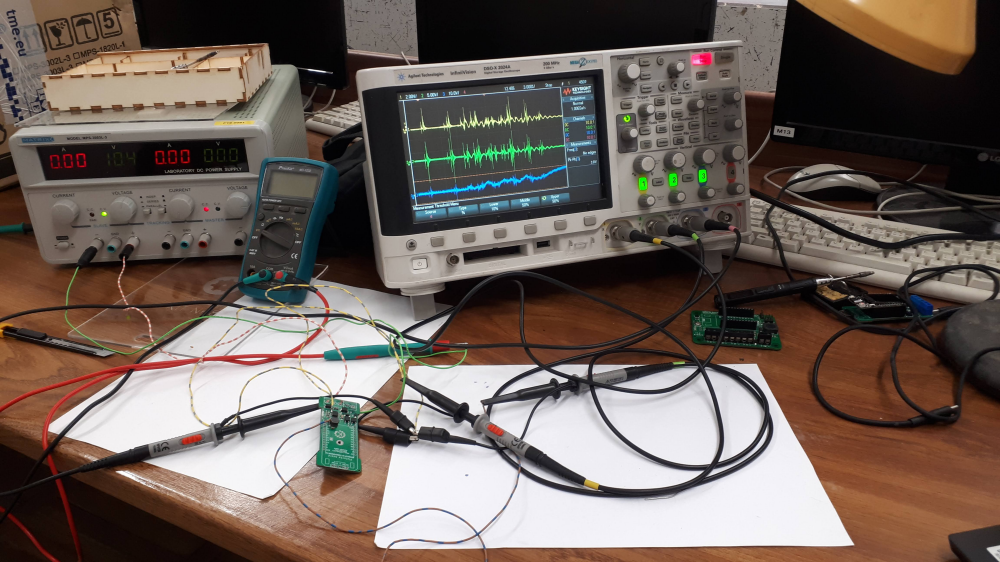
\includegraphics[width=\textwidth]{img/Testovani.png}
    \caption{Testování senzoru}
    \label{fig:SenzorNaStroji}
\end{figure}

%SECTION
\section{Testování ve firmě}
V~bodě kdy byly odladěny chyby jsem systém nasadil na dva pletací stroje.
Nově nasbíraná data byla již reálná a~dalo se na nich postavit nové testování.
Senzory jsem tedy nechal několik dní sbírat údaje o~upletených ponožkách a~následně jsem nad nimi spustil generování uživatelsky čitelných dat.

Od půlky prosince 2020 probíhá dlouhodobé testování bez zásahu do vygenerovaných dat. Naměřené údaje pravidelně stahuji a~kontroluji jejich správnost.

\newpage


% \chapter{Nasazení}
Lorem ipsum dolor sit amet, consectetur adipiscing elit.
Aliquam nunc magna, sollicitudin id leo eu, viverra congue risus.
Aliquam consequat ipsum ut erat placerat consequat nec at diam. 
Aenean est odio, molestie sit amet nunc in, pretium luctus elit. 
Donec imperdiet orci vel porttitor placerat. 
Proin ut hendrerit elit, ultricies accumsan urna. 
Vivamus condimentum lorem viverra lectus finibus, nec volutpat turpis auctor.
Cras quis felis non lorem consectetur interdum eu eu sem. 
Proin sit amet feugiat metus. 
Ut vitae orci a enim vestibulum porta. 



%SECTION
\section{Nasazení ve firmě}
Lorem ipsum dolor sit amet, consectetur adipiscing elit.
Aliquam nunc magna, sollicitudin id leo eu, viverra congue risus.
Aliquam consequat ipsum ut erat placerat consequat nec at diam. 
Aenean est odio, molestie sit amet nunc in, pretium luctus elit. 
Donec imperdiet orci vel porttitor placerat. 
Proin ut hendrerit elit, ultricies accumsan urna. 
Vivamus condimentum lorem viverra lectus finibus, nec volutpat turpis auctor.
Cras quis felis non lorem consectetur interdum eu eu sem. 
Proin sit amet feugiat metus. 
Ut vitae orci a enim vestibulum porta. 


\subsection{Zpětná vazba}
Lorem ipsum dolor sit amet, consectetur adipiscing elit.
Aliquam nunc magna, sollicitudin id leo eu, viverra congue risus.
Aliquam consequat ipsum ut erat placerat consequat nec at diam. 
Aenean est odio, molestie sit amet nunc in, pretium luctus elit. 
Donec imperdiet orci vel porttitor placerat. 
Proin ut hendrerit elit, ultricies accumsan urna. 
Vivamus condimentum lorem viverra lectus finibus, nec volutpat turpis auctor.
Cras quis felis non lorem consectetur interdum eu eu sem. 
Proin sit amet feugiat metus. 
Ut vitae orci a enim vestibulum porta. 




\newpage
\chapter{Zpětná vazba majitele firmy}
Systém Pletačka IoT funguje v~naší firmě ROTEX Vysočina již 3~měsíce a~pomáhá při~každodenním provozu analyzovat chod strojů.
Díky sběru dat on-line z~pletacího stroje je vše velmi rychlé a~efektivní.
Hlavním přínosem tohoto systému je jednoduché porovnávání pracovních směn, což nám umožňuje rychle analyzovat průběh výroby u~každého stroje.
Systém také využíváme k~vytváření výrobních statistik a~ke kontrole poruchovosti strojů.

{\raggedleft Za firmu Karel Krejčí\par}



\newpage


\chapter*{Závěr}

Cílem této práce bylo navrhnout ucelený systém, který dokáže:

\begin{itemize}
    \item počítat upletené ponožky
    \item zjišťovat poruchovost strojů
    \item porovnávat jednotlivé pracovní směny
    \item monitorovat průběh výroby
\end{itemize}

Všechny tyto vytyčené cíle se mi podařilo splnit. Systém nadále běží ve firmě ROTEX Vysočina s.r.o \cite{ROTEX} a~pomáhá v~běžném provozu.
Můj systém se stal nedílnou součástí výrobního procesu a~analyzuje průběh výroby.

Systém mám k~1. únoru 2021 nasazen na deseti pletacích strojích a~po dobu provozu zaznamenal již přes padesát tisíc upletených ponožek.
Celý systém je nasazený krátkou dobu, abych dokázal porovnat produktivitu před nasazením tohoto systému s~daty po nasazení.

Velkým přínosem pro firmu je porovnávání pracovních směn, díky kterým zaměstnavatel ihned vidí rozdíly mezi produktivitou práce v~daném čase.

Díky SOČ jsem se naučil navrhovat plošné spoje, rozšířil jsem si obzory v~elektronice a při vývoji jsem si vyzkoušel práci s měřícími přístroji. 
Také jsem se naučil programovat v~jazyce PHP a~vytvářet komplexní webové systémy.

V~budoucnu bych chtěl tento systém rozšířit na všechny pletací stroje a~pokrýt tak celou výrobnu.
Taktéž pokračuji na vylepšování webové aplikace a~plánuji ji rozšířit o~další funkce.
Jde například o~export dat do tabulek.

Tuto práci můžete najít na adrese: \url{https://github.com/JakubAndrysek/SOC-Integrace-do-prumyslu-4.0/blob/master/text.pdf}.

Všechny zdrojové kódy a DPS k projektu jsou k dispozici na \url{https://github.com/Pletacka-IoT} pod MIT licencí.


\newpage

\newpage



\appendix
\addcontentsline{toc}{chapter}{Přílohy}


\chapter{}


\begin{figure}[htbp]
    \centering
    % 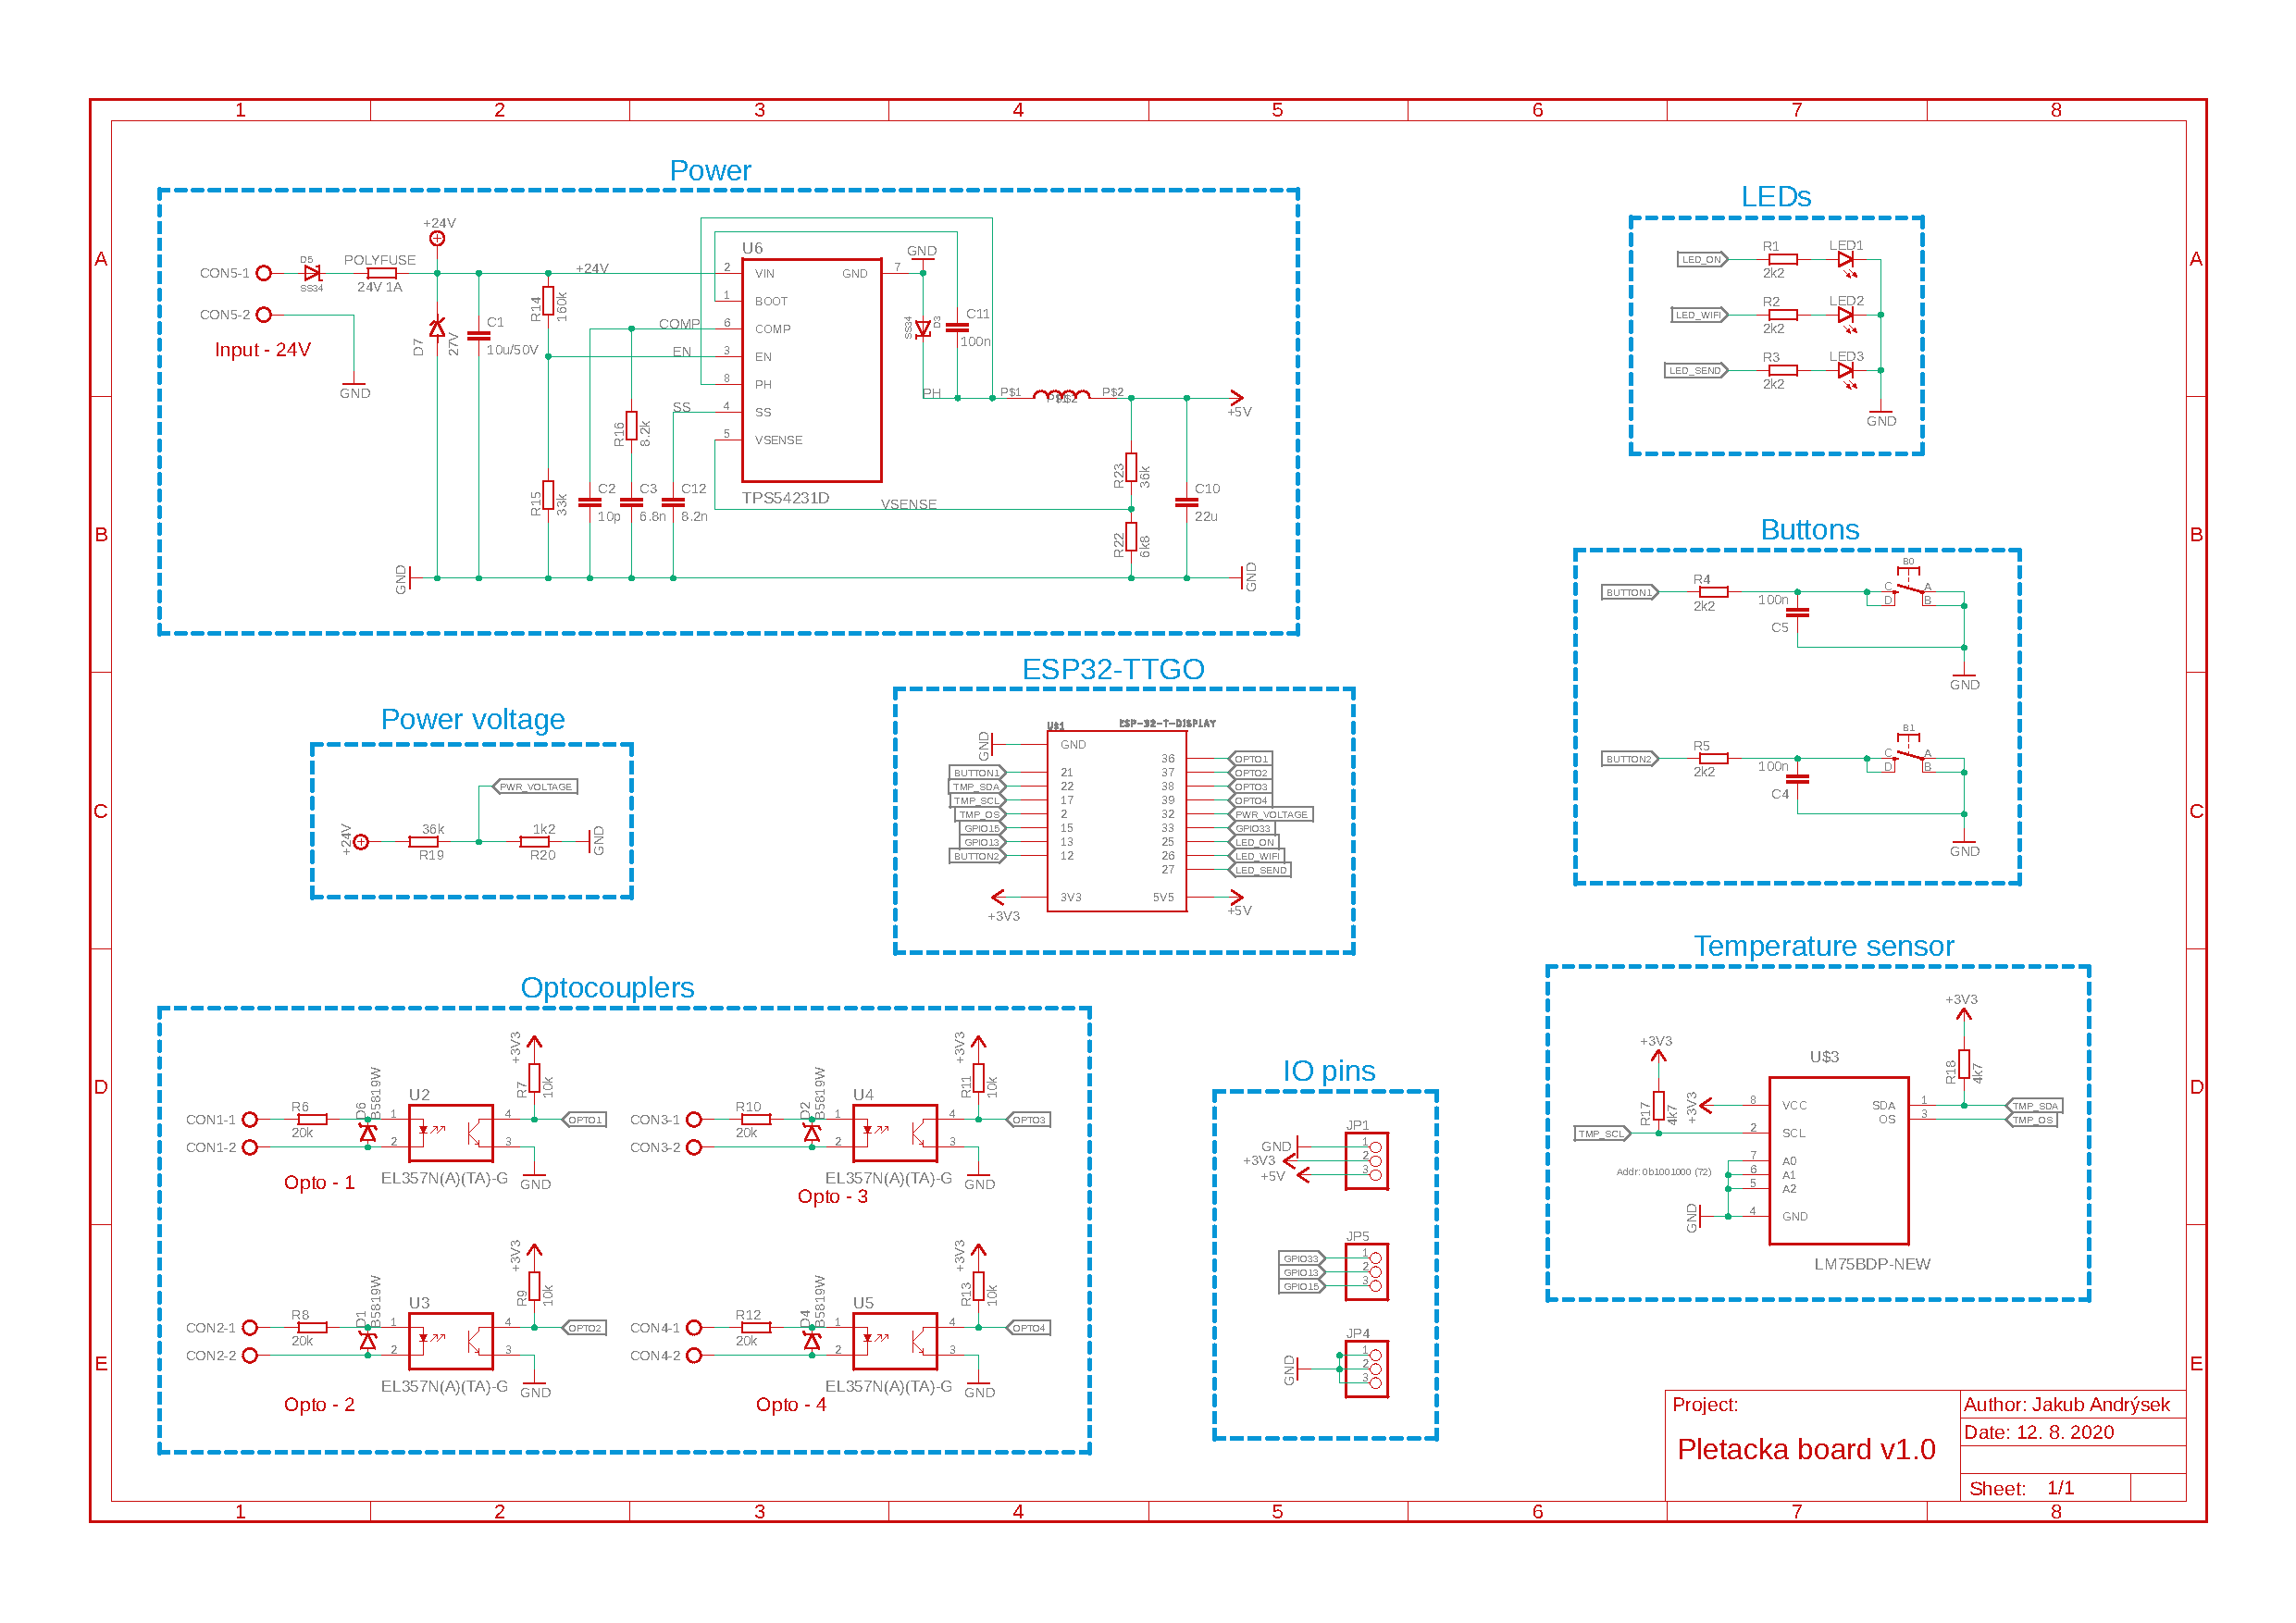
\includegraphics[scale=0.3]{DATASHEET/Pletacka_board_v1.pdf}
    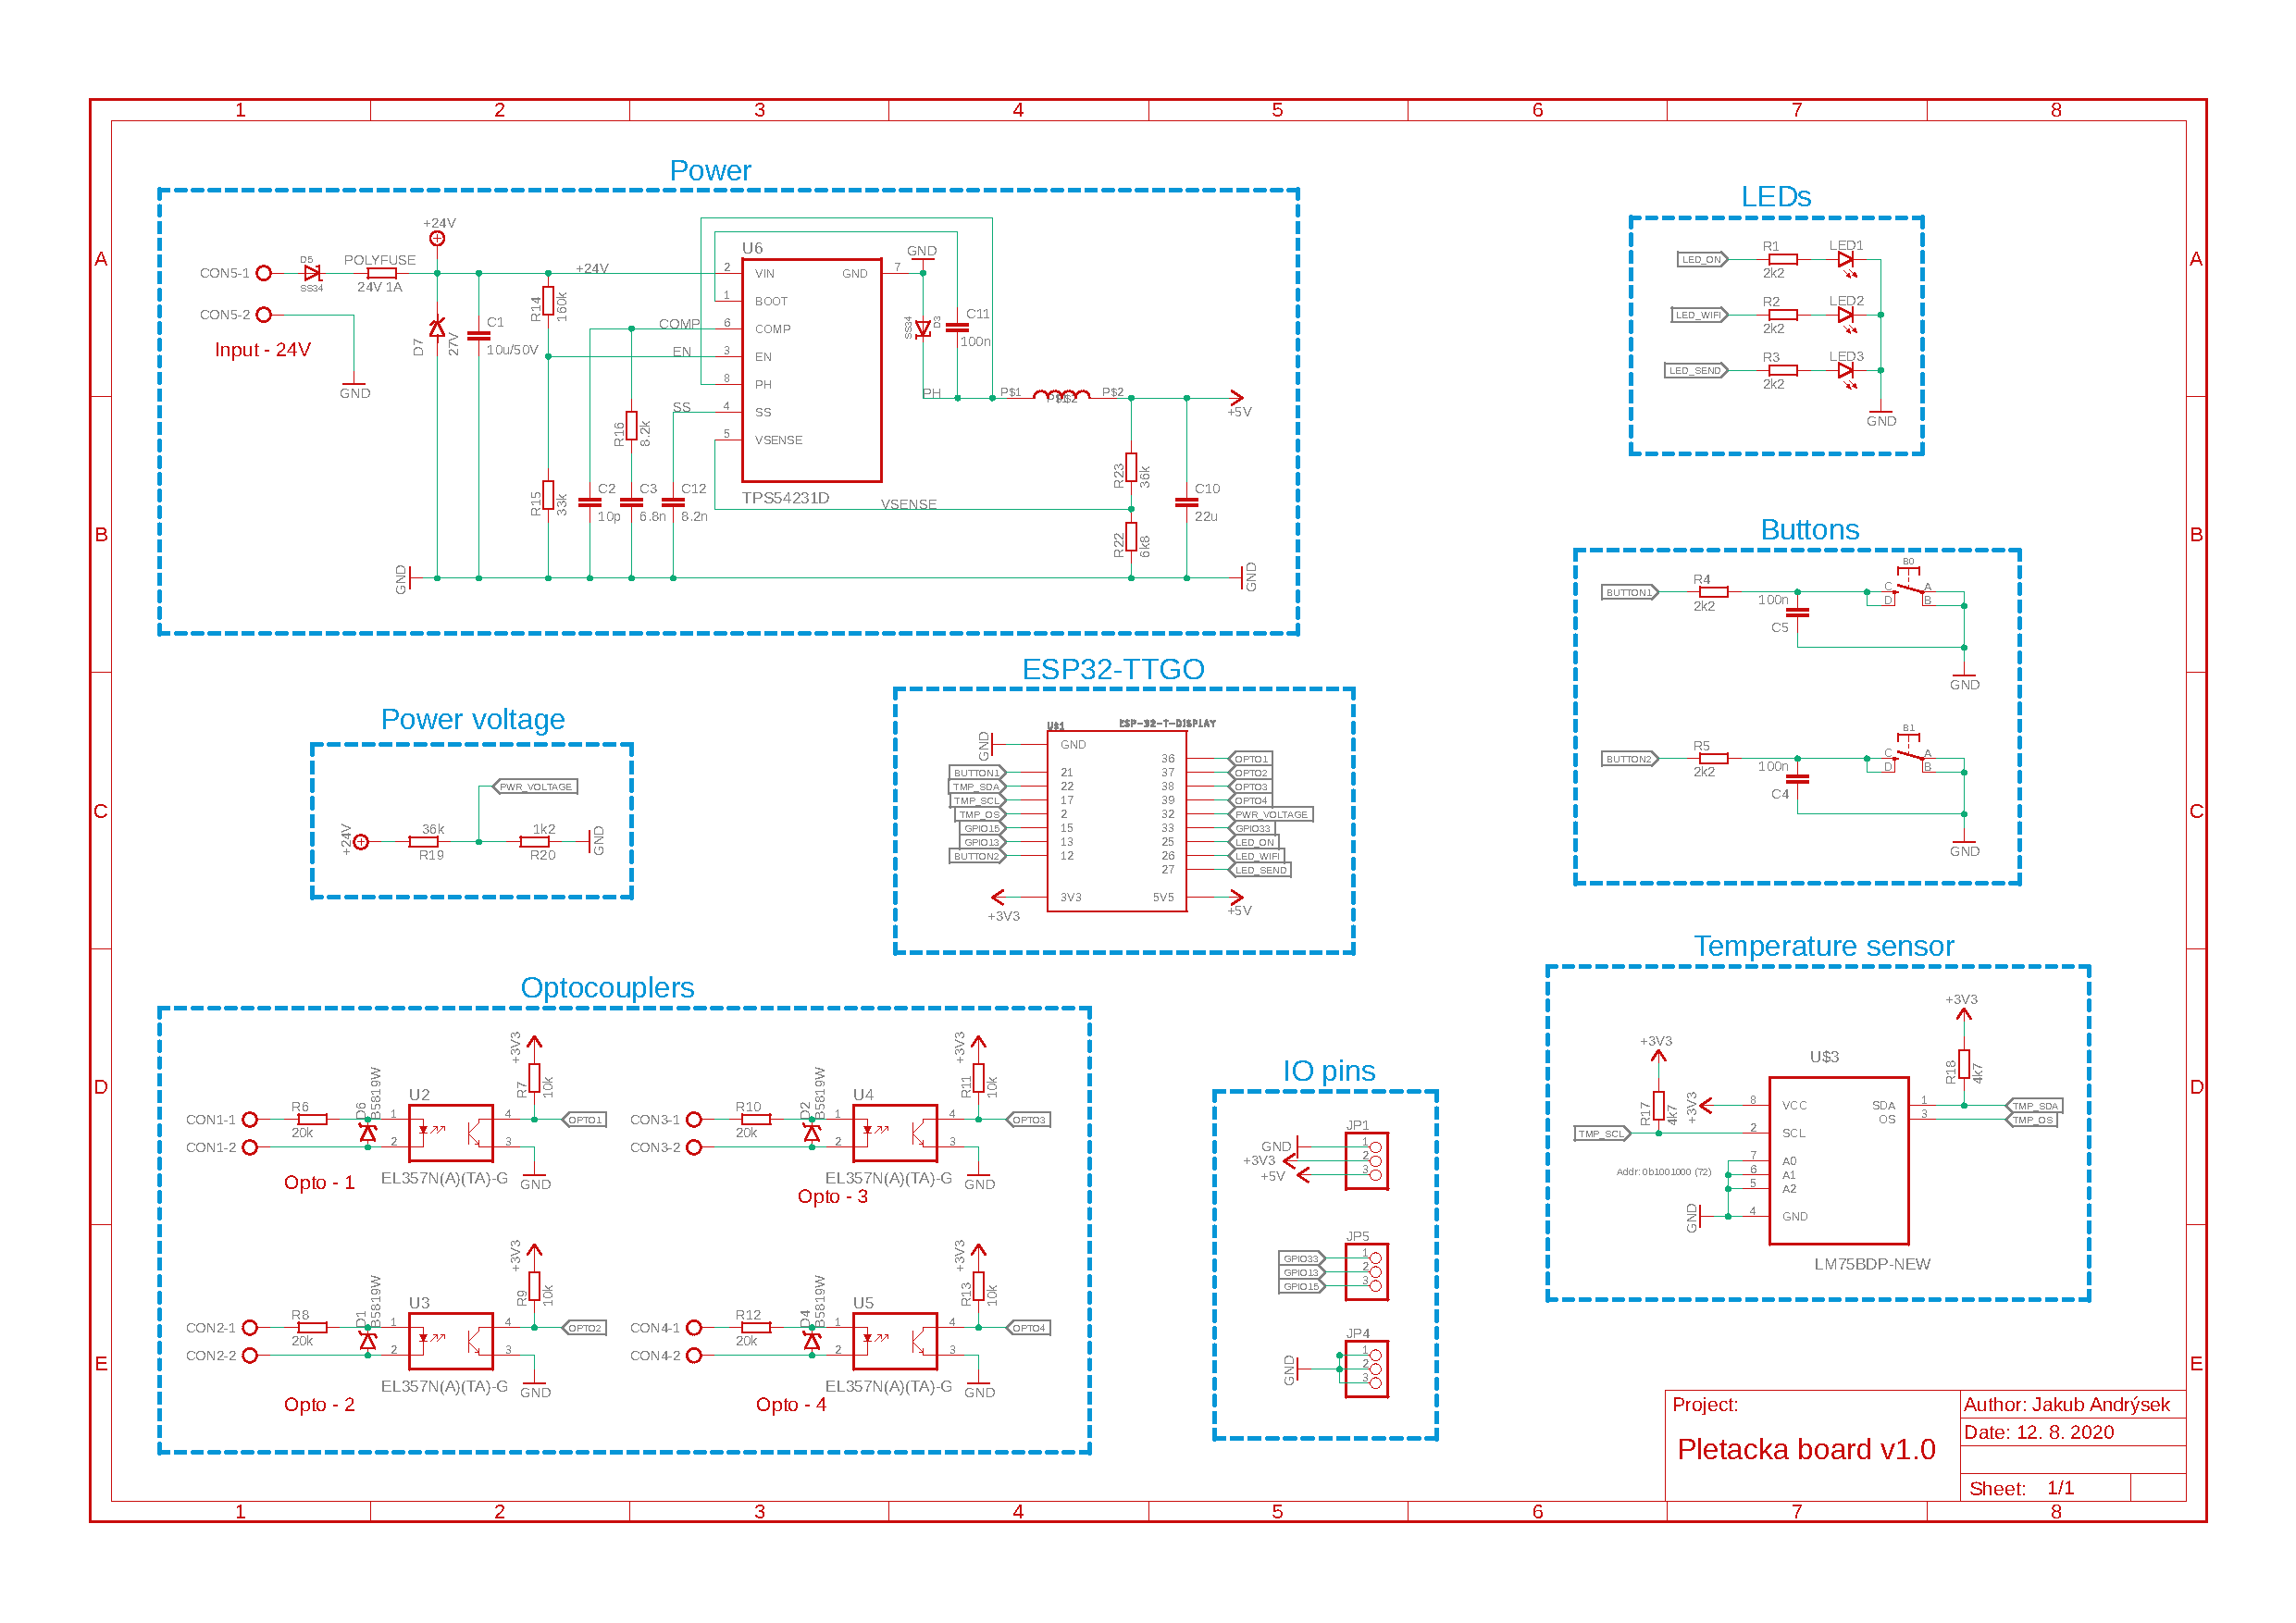
\includegraphics[width=\textwidth]{DATASHEET/Pletacka_board_v1.pdf}
    \caption{Schéma senzoru 1. verze}
    \label{fig:Schemav1}
\end{figure}


\begin{figure}[htbp]
    \centering
    % 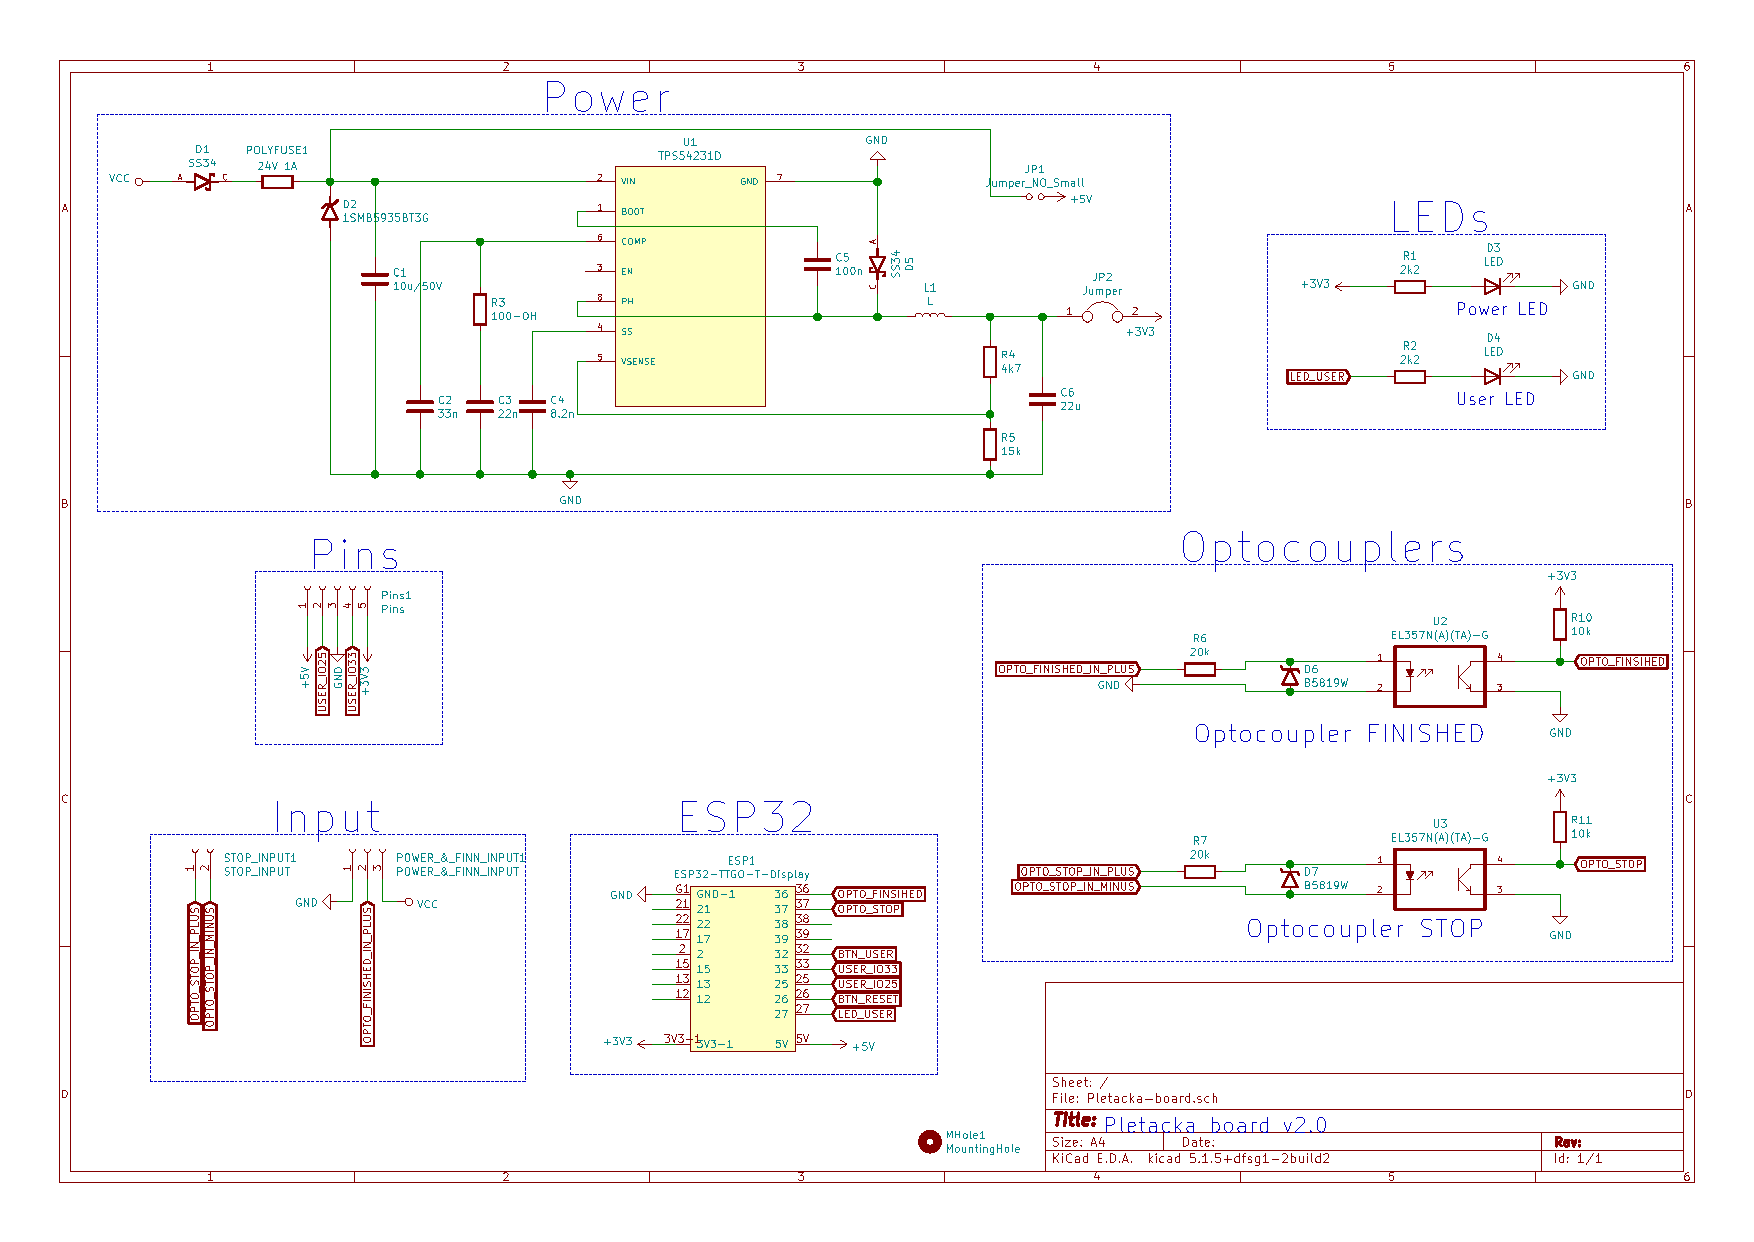
\includegraphics[scale=0.5]{DATASHEET/Pletacka_board_v2.pdf}
    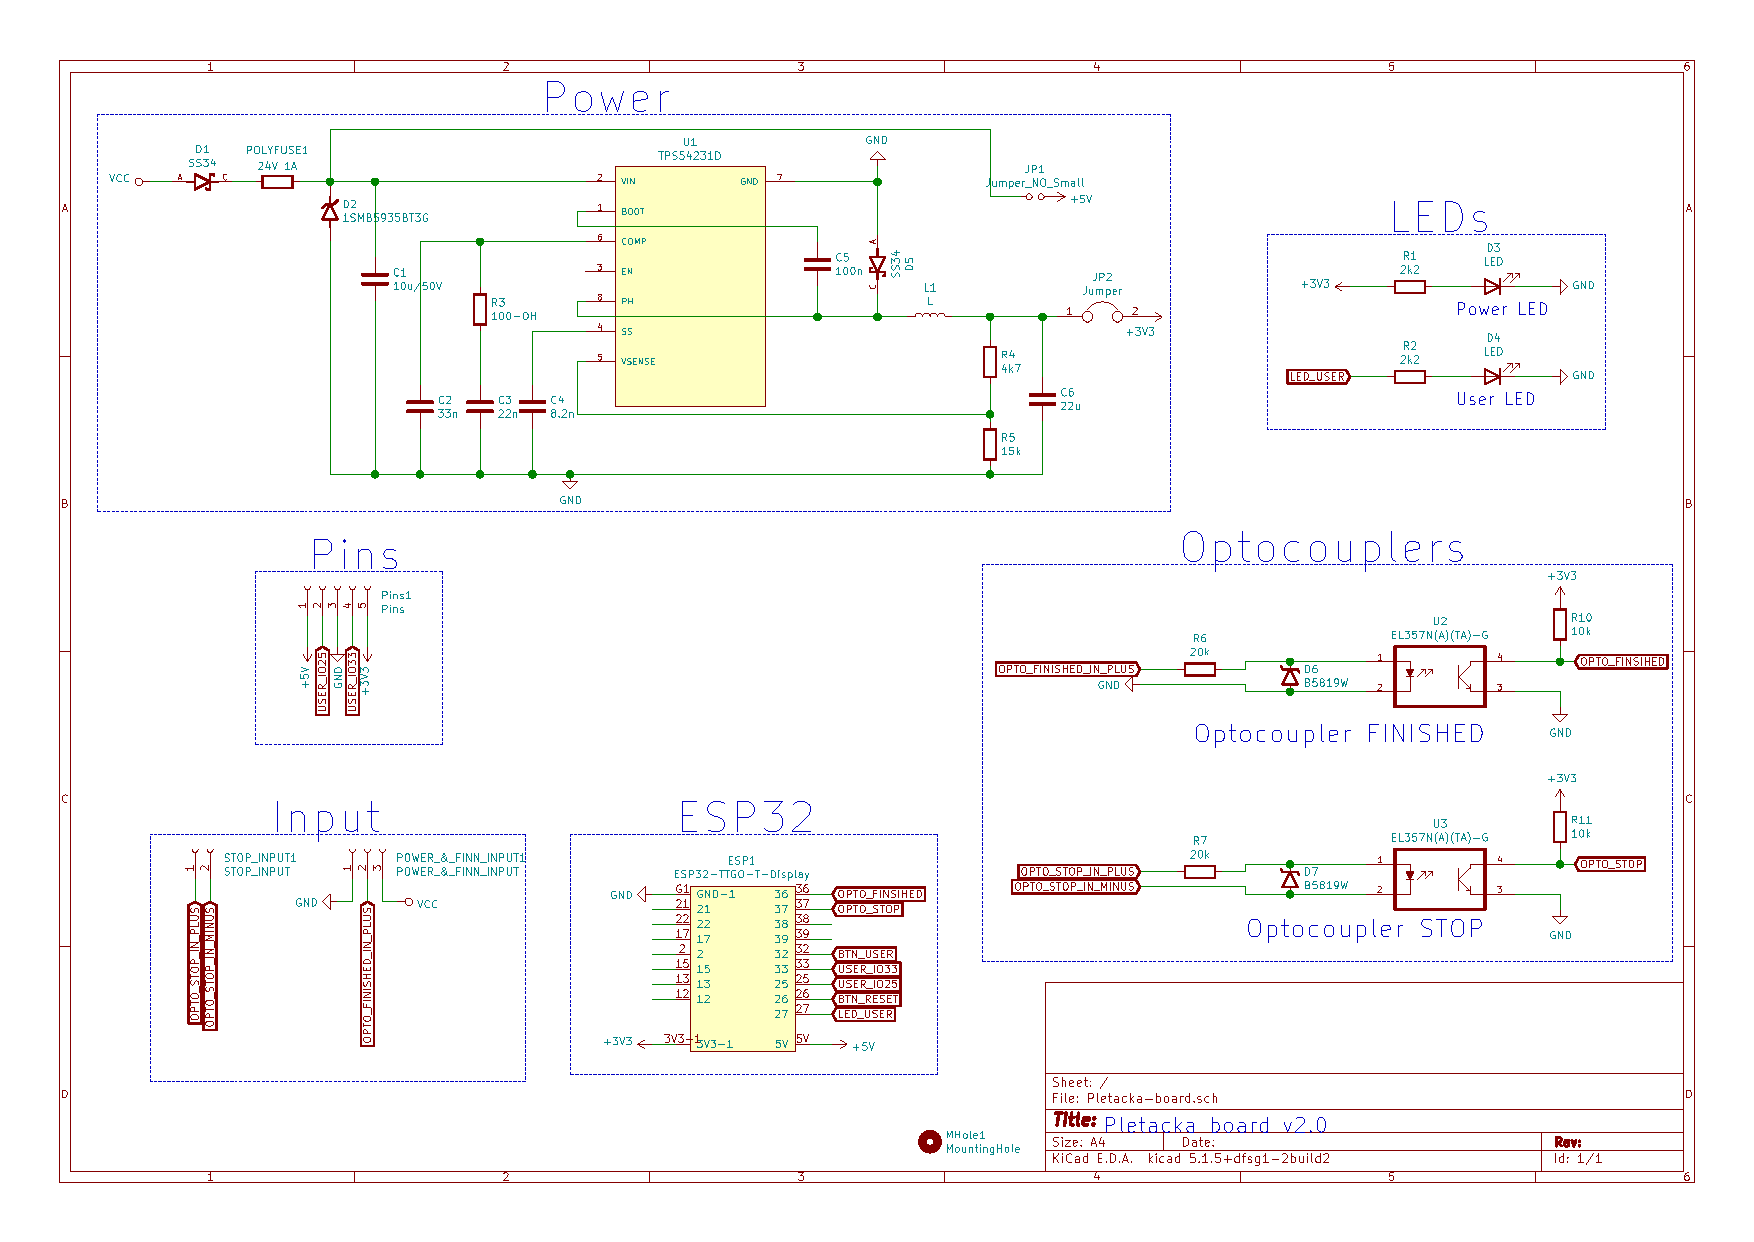
\includegraphics[width=\textwidth]{DATASHEET/Pletacka_board_v2.pdf}
    \caption{Schéma senzoru 2. verze}
    \label{fig:Schemav1}
\end{figure}

\begin{figure}[htbp]
    \centering
    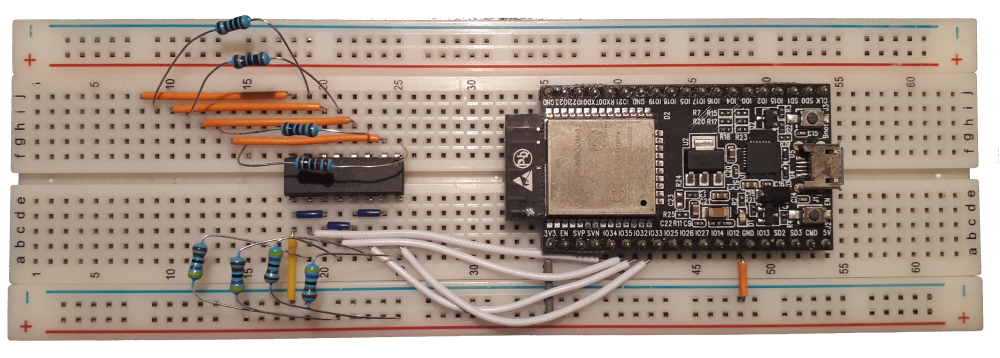
\includegraphics[width=\textwidth]{img/nepajivePole.png}
    \caption{Testování funkčnosti zapojení}
    \label{fig:Pletarna}
\end{figure}


\begin{figure}[htbp]
    \centering
    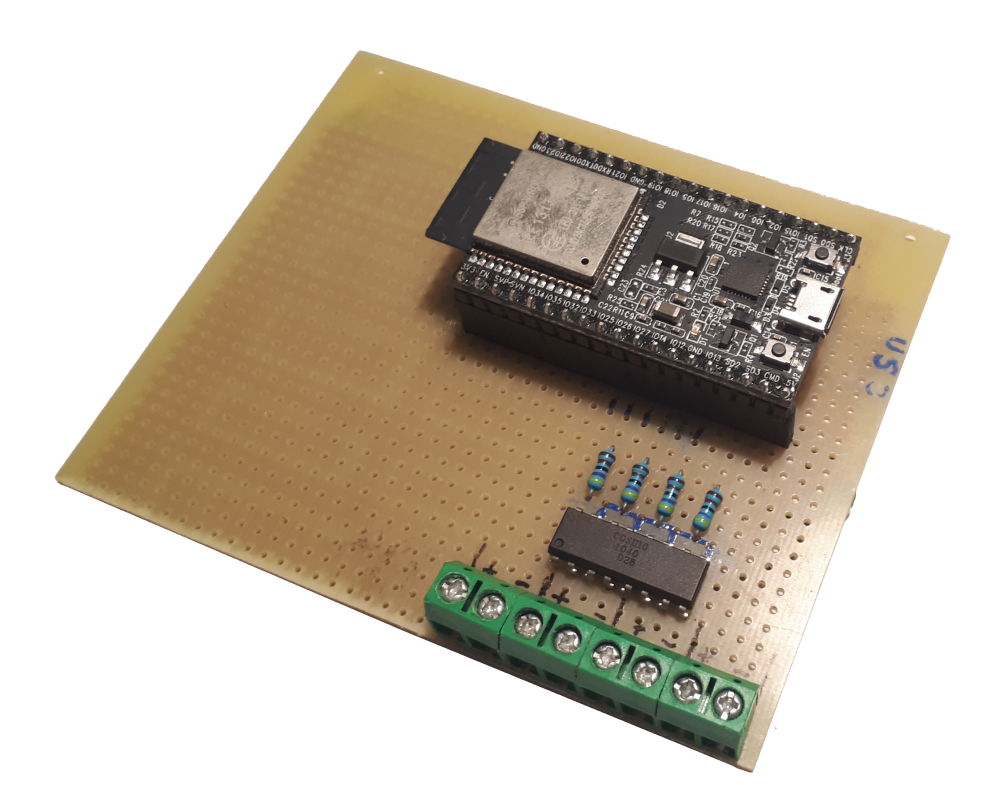
\includegraphics[width=0.8\textwidth]{img/testovaciSenzor.png}
    \caption{Testovací verze senzoru}
    \label{fig:testovaciSenzor}
\end{figure}


\begin{figure}[htbp]
    \centering
    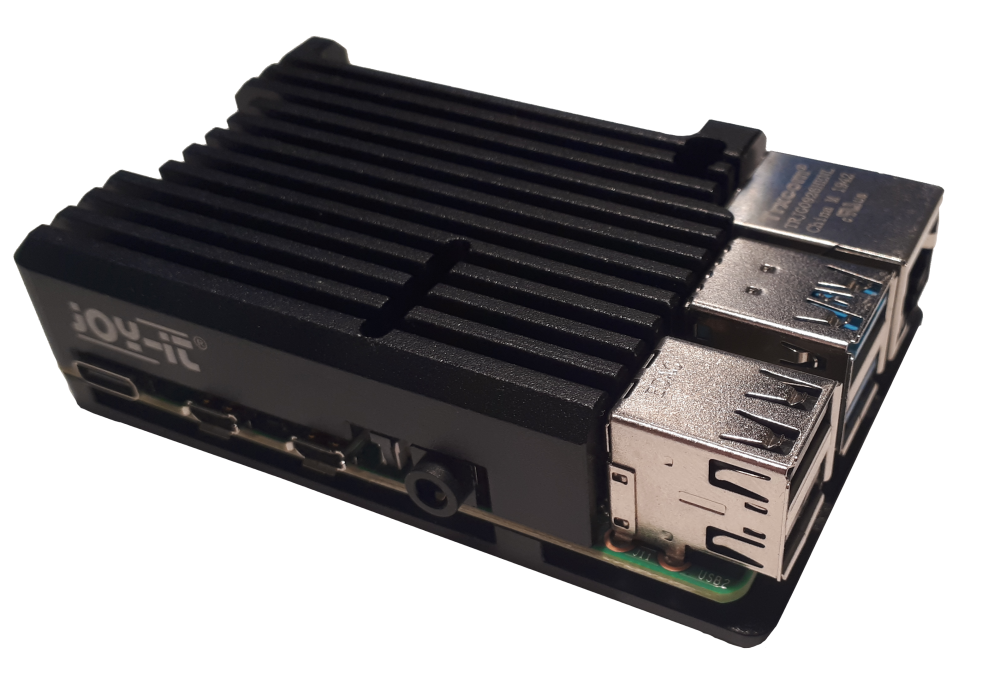
\includegraphics[width=0.8\textwidth]{img/malina.png}
    \caption{Webový server Raspberry Pi}
    \label{fig:malina}
\end{figure}


\begin{figure}[htbp]
    \centering
    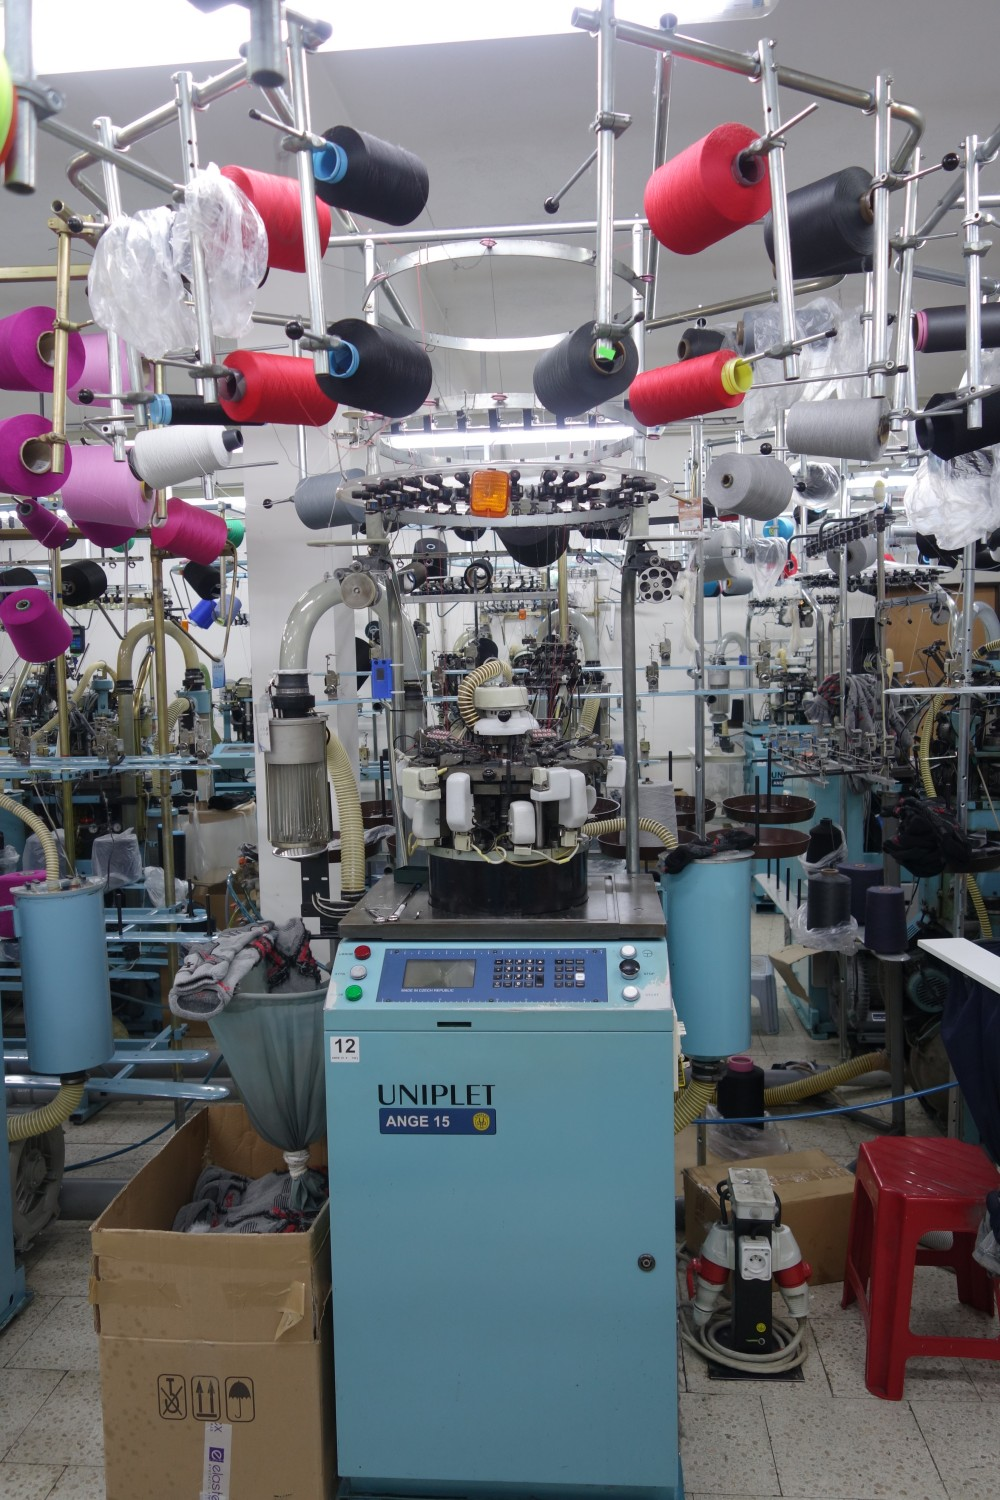
\includegraphics[width=0.9\textwidth]{img/pletacka.png}
    \caption{Pletací stroj}
    \label{fig:pletacka}
\end{figure}

\newpage



% \chapter{Senzory}
Lorem ipsum dolor sit amet, consectetur adipiscing elit.
Aliquam nunc magna, sollicitudin id leo eu, viverra congue risus.
Aliquam consequat ipsum ut erat placerat consequat nec at diam. 
Aenean est odio, molestie sit amet nunc in, pretium luctus elit. 
Donec imperdiet orci vel porttitor placerat. 
Proin ut hendrerit elit, ultricies accumsan urna. 
Vivamus condimentum lorem viverra lectus finibus, nec volutpat turpis auctor.
Cras quis felis non lorem consectetur interdum eu eu sem. 
Proin sit amet feugiat metus. 
Ut vitae orci a enim vestibulum porta. 


%SECTION
\section{Pletačka board v1.0}
Lorem ipsum dolor sit amet, consectetur adipiscing elit.
Aliquam nunc magna, sollicitudin id leo eu, viverra congue risus.
Aliquam consequat ipsum ut erat placerat consequat nec at diam. 
Aenean est odio, molestie sit amet nunc in, pretium luctus elit. 
Donec imperdiet orci vel porttitor placerat. 
Proin ut hendrerit elit, ultricies accumsan urna. 
Vivamus condimentum lorem viverra lectus finibus, nec volutpat turpis auctor.
Cras quis felis non lorem consectetur interdum eu eu sem. 
Proin sit amet feugiat metus. 
Ut vitae orci a enim vestibulum porta. 


\subsection{Hardware}
Lorem ipsum dolor sit amet, consectetur adipiscing elit.
Aliquam nunc magna, sollicitudin id leo eu, viverra congue risus.
Aliquam consequat ipsum ut erat placerat consequat nec at diam. 
Aenean est odio, molestie sit amet nunc in, pretium luctus elit. 
Donec imperdiet orci vel porttitor placerat. 
Proin ut hendrerit elit, ultricies accumsan urna. 
Vivamus condimentum lorem viverra lectus finibus, nec volutpat turpis auctor.
Cras quis felis non lorem consectetur interdum eu eu sem. 
Proin sit amet feugiat metus. 
Ut vitae orci a enim vestibulum porta. 


\subsection{Software}
Lorem ipsum dolor sit amet, consectetur adipiscing elit.
Aliquam nunc magna, sollicitudin id leo eu, viverra congue risus.
Aliquam consequat ipsum ut erat placerat consequat nec at diam. 
Aenean est odio, molestie sit amet nunc in, pretium luctus elit. 
Donec imperdiet orci vel porttitor placerat. 
Proin ut hendrerit elit, ultricies accumsan urna. 
Vivamus condimentum lorem viverra lectus finibus, nec volutpat turpis auctor.
Cras quis felis non lorem consectetur interdum eu eu sem. 
Proin sit amet feugiat metus. 
Ut vitae orci a enim vestibulum porta. 



%SECTION
\section{Pletačka board v2.0}
Lorem ipsum dolor sit amet, consectetur adipiscing elit.
Aliquam nunc magna, sollicitudin id leo eu, viverra congue risus.
Aliquam consequat ipsum ut erat placerat consequat nec at diam. 
Aenean est odio, molestie sit amet nunc in, pretium luctus elit. 
Donec imperdiet orci vel porttitor placerat. 
Proin ut hendrerit elit, ultricies accumsan urna. 
Vivamus condimentum lorem viverra lectus finibus, nec volutpat turpis auctor.
Cras quis felis non lorem consectetur interdum eu eu sem. 
Proin sit amet feugiat metus. 
Ut vitae orci a enim vestibulum porta. 


\subsection{Hardware}
Lorem ipsum dolor sit amet, consectetur adipiscing elit.
Aliquam nunc magna, sollicitudin id leo eu, viverra congue risus.
Aliquam consequat ipsum ut erat placerat consequat nec at diam. 
Aenean est odio, molestie sit amet nunc in, pretium luctus elit. 
Donec imperdiet orci vel porttitor placerat. 
Proin ut hendrerit elit, ultricies accumsan urna. 
Vivamus condimentum lorem viverra lectus finibus, nec volutpat turpis auctor.
Cras quis felis non lorem consectetur interdum eu eu sem. 
Proin sit amet feugiat metus. 
Ut vitae orci a enim vestibulum porta. 


\subsection{Software}
Lorem ipsum dolor sit amet, consectetur adipiscing elit.
Aliquam nunc magna, sollicitudin id leo eu, viverra congue risus.
Aliquam consequat ipsum ut erat placerat consequat nec at diam. 
Aenean est odio, molestie sit amet nunc in, pretium luctus elit. 
Donec imperdiet orci vel porttitor placerat. 
Proin ut hendrerit elit, ultricies accumsan urna. 
Vivamus condimentum lorem viverra lectus finibus, nec volutpat turpis auctor.
Cras quis felis non lorem consectetur interdum eu eu sem. 
Proin sit amet feugiat metus. 
Ut vitae orci a enim vestibulum porta. 



\newpage


% \chapter{Webový server}

!!!!!  Pletačka website !!!!!

Lorem ipsum dolor sit amet, consectetur adipiscing elit.
Aliquam nunc magna, sollicitudin id leo eu, viverra congue risus.
Aliquam consequat ipsum ut erat placerat consequat nec at diam. 
Aenean est odio, molestie sit amet nunc in, pretium luctus elit. 
Donec imperdiet orci vel porttitor placerat. 
Proin ut hendrerit elit, ultricies accumsan urna. 
Vivamus condimentum lorem viverra lectus finibus, nec volutpat turpis auctor.
Cras quis felis non lorem consectetur interdum eu eu sem. 
Proin sit amet feugiat metus. 
Ut vitae orci a enim vestibulum porta. 



\section{Struktura projektu}
Lorem ipsum dolor sit amet, consectetur adipiscing elit.
Aliquam nunc magna, sollicitudin id leo eu, viverra congue risus.
Aliquam consequat ipsum ut erat placerat consequat nec at diam. 
Aenean est odio, molestie sit amet nunc in, pretium luctus elit. 
Donec imperdiet orci vel porttitor placerat. 
Proin ut hendrerit elit, ultricies accumsan urna. 
Vivamus condimentum lorem viverra lectus finibus, nec volutpat turpis auctor.
Cras quis felis non lorem consectetur interdum eu eu sem. 
Proin sit amet feugiat metus. 
Ut vitae orci a enim vestibulum porta. 

\section{Uživatelské rozhraní}
Lorem ipsum dolor sit amet, consectetur adipiscing elit.
Aliquam nunc magna, sollicitudin id leo eu, viverra congue risus.
Aliquam consequat ipsum ut erat placerat consequat nec at diam. 
Aenean est odio, molestie sit amet nunc in, pretium luctus elit. 
Donec imperdiet orci vel porttitor placerat. 
Proin ut hendrerit elit, ultricies accumsan urna. 
Vivamus condimentum lorem viverra lectus finibus, nec volutpat turpis auctor.
Cras quis felis non lorem consectetur interdum eu eu sem. 
Proin sit amet feugiat metus. 
Ut vitae orci a enim vestibulum porta. 

\section{Backend}
Lorem ipsum dolor sit amet, consectetur adipiscing elit.
Aliquam nunc magna, sollicitudin id leo eu, viverra congue risus.
Aliquam consequat ipsum ut erat placerat consequat nec at diam. 
Aenean est odio, molestie sit amet nunc in, pretium luctus elit. 
Donec imperdiet orci vel porttitor placerat. 
Proin ut hendrerit elit, ultricies accumsan urna. 
Vivamus condimentum lorem viverra lectus finibus, nec volutpat turpis auctor.
Cras quis felis non lorem consectetur interdum eu eu sem. 
Proin sit amet feugiat metus. 
Ut vitae orci a enim vestibulum porta. 

\section{API}
Lorem ipsum dolor sit amet, consectetur adipiscing elit.
Aliquam nunc magna, sollicitudin id leo eu, viverra congue risus.
Aliquam consequat ipsum ut erat placerat consequat nec at diam. 
Aenean est odio, molestie sit amet nunc in, pretium luctus elit. 
Donec imperdiet orci vel porttitor placerat. 
Proin ut hendrerit elit, ultricies accumsan urna. 
Vivamus condimentum lorem viverra lectus finibus, nec volutpat turpis auctor.
Cras quis felis non lorem consectetur interdum eu eu sem. 
Proin sit amet feugiat metus. 
Ut vitae orci a enim vestibulum porta. 


\newpage


% \chapter{Podpůrný server}

!!!Pletačka python server!!!!!!
Lorem ipsum dolor sit amet, consectetur adipiscing elit.
Aliquam nunc magna, sollicitudin id leo eu, viverra congue risus.
Aliquam consequat ipsum ut erat placerat consequat nec at diam. 
Aenean est odio, molestie sit amet nunc in, pretium luctus elit. 
Donec imperdiet orci vel porttitor placerat. 
Proin ut hendrerit elit, ultricies accumsan urna. 
Vivamus condimentum lorem viverra lectus finibus, nec volutpat turpis auctor.
Cras quis felis non lorem consectetur interdum eu eu sem. 
Proin sit amet feugiat metus. 
Ut vitae orci a enim vestibulum porta. 



\section{Komunikace se senzory}
Lorem ipsum dolor sit amet, consectetur adipiscing elit.
Aliquam nunc magna, sollicitudin id leo eu, viverra congue risus.
Aliquam consequat ipsum ut erat placerat consequat nec at diam. 
Aenean est odio, molestie sit amet nunc in, pretium luctus elit. 
Donec imperdiet orci vel porttitor placerat. 
Proin ut hendrerit elit, ultricies accumsan urna. 
Vivamus condimentum lorem viverra lectus finibus, nec volutpat turpis auctor.
Cras quis felis non lorem consectetur interdum eu eu sem. 
Proin sit amet feugiat metus. 
Ut vitae orci a enim vestibulum porta. 

\section{Aktualizace senzorů}
Lorem ipsum dolor sit amet, consectetur adipiscing elit.
Aliquam nunc magna, sollicitudin id leo eu, viverra congue risus.
Aliquam consequat ipsum ut erat placerat consequat nec at diam. 
Aenean est odio, molestie sit amet nunc in, pretium luctus elit. 
Donec imperdiet orci vel porttitor placerat. 
Proin ut hendrerit elit, ultricies accumsan urna. 
Vivamus condimentum lorem viverra lectus finibus, nec volutpat turpis auctor.
Cras quis felis non lorem consectetur interdum eu eu sem. 
Proin sit amet feugiat metus. 
Ut vitae orci a enim vestibulum porta. 
orci a enim vestibulum porta. 



\newpage



\printbibliography[title=Literatura]

\addcontentsline{toc}{chapter}{Literatura}

\listoffigures
\addcontentsline{toc}{section}{Seznam obrázků}

\listoftables
\addcontentsline{toc}{section}{Seznam tabulek}

\end{document}

% Uprava na tvrde mezery "\b([aiouksvz]) " (i s tou mezerou na konci) => "$1~"
